% !TeX spellcheck = fr-toutesvariantes
\documentclass[12pt]{report}
\usepackage{longtable}
\usepackage[table,xcdraw]{xcolor}
\usepackage[utf8]{inputenc}
\usepackage[T1]{fontenc}
\usepackage[francais]{babel}
\usepackage{fixltx2e}
\usepackage{charter}
\usepackage{amsmath}
\usepackage{float}
\usepackage{wrapfig}
\usepackage{graphicx}
\usepackage{soul}
\usepackage[colorlinks=true, linkcolor=blue]{hyperref}
\usepackage[a4paper, width=150mm, top=25mm, bottom=25mm]{geometry}
\usepackage{parskip}
\usepackage{enumitem}
\usepackage[final]{pdfpages}
\usepackage[linguistics]{forest}
%\usepackage{titlesec}
\usepackage{listings}
\usepackage[final]{pdfpages}
\usepackage[font=small,labelfont=bf]{caption} % Required for specifying captions to tables and figures
\setlist[itemize]{label=\textbullet}
\usepackage[linesnumbered,algoruled,french,onelanguage]{algorithm2e}
\usepackage{url}
\usepackage{amsmath}
\usepackage{algorithmicx}
\usepackage{xcolor}
\usepackage{multirow}
\usepackage[noend]{algpseudocode}
\usepackage{tabularx}  % for tabularx
% to make cells in table have decent spacing
\usepackage{diagbox}
\usepackage{color, colortbl}
\usepackage{array}
\usepackage{tabularx} % in the preamble
\usepackage{csvsimple}
\usepackage{geometry}
\geometry{
	a4paper,
	total={170mm,257mm},
	left=20mm,
	top=20mm,
}
\usepackage{wrapfig}

\newcolumntype{L}[1]{>{\raggedright\let\newline\\\arraybackslash\hspace{0pt}}m{#1}}
\newcolumntype{C}[1]{>{\centering\let\newline\\\arraybackslash\hspace{0pt}}m{#1}}
\newcolumntype{R}[1]{>{\raggedleft\let\newline\\\arraybackslash\hspace{0pt}}m{#1}}
\lstset{
	language=Python,                   % choix du langage (de programmation).
	keywordstyle=\color{blue},      % choix de la couleur des mots clés.
	stringstyle=\color{red},        % choix de la couleur des string.
	commentstyle=\color{green},     % choix de la couleur des commentaire.
	basicstyle=\normalsize,     % taille de la police du code
	% numbers=left,                   % placer le numéro de chaque ligne à gauche (on peut choisir à droite, ou ne pas mettre cette option pour aucun numéro de ligne).
	numberstyle=\normalsize,        % taille de la police des numéros.
	numbersep=0pt,                  % distance entre le code et sa numérotation.
	showstringspaces=false,         % pour ne pas afficher les espaces comme des caractères .
	breaklines=true,                % couper la ligne si la ligne du code est trop longue.
}
\def \hfillx {\hspace*{-\textwidth} \hfill}


\begin{document}
\hypersetup{hidelinks}

\includepdf[pages=1]{Page_garde.pdf} 
\tableofcontents

\pagenumbering{arabic}
\newpage

%%%Include Part 1
\part{Approche par espace des états}\label{part1} 

\chapter{Introduction : }
\section{Problématique : }
\paragraph{}
Dans ce TP, nous allons tenter d'implémenter et de comparer plusieurs méthodes aveugles, dites aussi \textbf{à base d'espace d'états}, Pour la résolution du problème de satisfiabilité, plus communément appelé \textbf{Problème SAT}, Ce travail est aussi une application directe des différentes méthodes vues durant le premier semestre en ce qui concerne la \textbf{Résolution de problèmes}, mais aussi la \textbf{Complexité des algorithmes et les structures de données}.
\section{Définitions}
\paragraph{}
Avant de rentrer dans les détails de la résolution du problème, nous devons d'abord définir ce qu'est le problème SAT, ainsi que les différentes méthodes utilisées pour sa résolution dans ce TP.
\subsection{Problème SAT}
\paragraph{}
Dans le domaine de l'informatique et de la logique, le problème de satisfiablité (\textbf{SAT}), est un problème de décision où il s'agit d'assigner des valeurs de vérité à des variables tel qu'un ensemble de clauses en forme normale conjonctives FNC\footnote{Une conjonction de disjonction de litérraux} préalablement défini soit satisfiable, en d'autres termes, que toutes les clauses soient vraies pour les mêmes valeurs de vérité de leurs litérraux\footnote{Une variables logique ou bien sa négation}, ce problème est le premier à avoir été démontré comme étant \textbf{NP-Complet}, et cela par \href{https://en.wikipedia.org/wiki/Stephen_Cook}{Stephen Cook} dans \cite{cook}, et qui a donc posé les fondements de l'informathique théoriques et de la théorie de la complexité.
\newpage
\subsection{Stratégie de recherche dans l'espace des états}
En cosidérant l'espace de recherche comme étant une arborescence, dont les noeuds sont les differents états du problème, nous pouvons classer les différentes stratégies de recherches en deux grandes catégories :
\subsection{Stratégie de rercherche aveugle}
\paragraph{}Cette catégories englobe les stratégies ou il est question de passer par toutes les solutions et les tester une à une, dans ce TP nous nous intéresserons plus particulièrement aux algortihmes/methodes suivant(es) :  
\subsubsection{Par prodonfeur d'abord (DFS)}\label{DFSdef}
\paragraph{}
L'algorithme de parcours en profondeur d'abord consiste à visité un noeud de départ (souvent appelé \textbf{racine}), puis visite le premier sommet voisin(ou \textbf{successeur}) jusqu'à ce qu'une profondeur limite soit atteinte ou bien qu'il n'y ait plus de voisin à developper, une variante de cet algorithme utilise deux ensemble \textbf{Open} et \textbf{Closed} qui représentent réspectivement l'ensemble des noeuds du graphe qui n'ont pas encore étés developpés et ceux déjà développés, cet ajout permet à l'algorithme d'éviter de boucler indéfiniment sur un ensemble de noeuds.
\begin{itemize}
	\item Complexité temporelle : $O(2^{N})$
	\item Complexité spatiale : $O(2m)$ avec $m$=nombre de litéraux 
\end{itemize}
\subsubsection{En Largeur d'abord (BFS)}\label{BFSdef}
\paragraph{}
Cet algorithme diffère de son prédecesseur par le fait qu'il visite tous les voisins(\textbf{successeurs}) d'un noeud avant de passer au noeud suivant, ce qui revient à gérer l'ajout et la suppression de l'ensemble Open comme une file, donc en mode \textbf{FIFO} (En supposant bien sûr qu'on dispose des deux ensembles open et closed), cet approche permet de sauvegarder tous les noeuds précèdemment visité durant la recherche, ce qui peut causer un débordement de la mémoire lors de l'exécution sur machine(Ce point sera rediscuté dans \ref{BreadthIssue} page \pageref{BreadthIssue} et \ref{BreadthIssueExperience} page \pageref{BreadthIssueExperience} et \ref{BreadthIssueCompare} page \pageref{BreadthIssueCompare})

\begin{itemize}
	\item Complexité temporelle : $O(2^{N})$
	\item Complexité spatiale : $O(2^N)$ avec $N$=nombre de litéraux 
\end{itemize}
\newpage
\subsubsection{Par coût uniforme}\label{DijkstraDef}
\paragraph{}
Le principe est simple, au fur et à mesur que l'algorithme avance et développe des noeuds, il garde en mémoire le coût\footnote[1]{Fonction retournant le cout pour passer du noeud de départ(la racine) au noeud courant}, le noeud qui sera ensuite choisi sera celui dont le coût accumulé est le plus bas, assurant ainsi de toujours choisir le chemin le plus optimal, si le coût pour passer d'un noeud à n'importe quel autre de ses voisins est le même quelque soit le neoud, l'algorithme est alors équivalent à celui de la recherche en largeur d'abord
\begin{itemize}
	\item Complexité temporelle : $O(2^{N})$
	\item Complexité spatiale : $O(2^N)$ avec $N$=nombre de litéraux  
\end{itemize}
\subsection{Stratégie de rercherche guidée}
Cette catégorie englobe quant à elle les stratégies ou il est question de parcourir une plus petite partie de l'espace de recherche dans l'espoir de trouver la solution optimal en un temps plus réduit, les algortihmes sont les suivants : 
\subsubsection{Recherche gloutonne (Greedy algorithm)}\label{GreedyDef}
\paragraph{}
Cet algorithme est basé sur la notion d'heuristique\footnote[1]{Une fonction d'éstimation de la distance séparant le noeud courant au but }, au lieu de parcourir de façon "naïve" l'ensemble des noeuds dans l'espace de recherche, il choisit a chaque itérration sur l'ensemble \textbf{open} le noeud le plus \textbf{prometteur} en terme de distance par rapport au but recherché.
\begin{itemize}
	\item Complexité temporelle : $O(2^{N})$
	\item Complexité spatiale : $O(2^N)$ avec $N$=nombre de litéraux 
\end{itemize}
\subsubsection{Algorithme A*}\label{AstarDef}
\paragraph{}
Contrairement aux précedents algorithmes de recherche qui effectuaient une recherche de façon "naîve", l'algorithme \textbf{A* }propose une vision un peu nouvelle, il utilise la notion de coût et celle d'heuristique, la fonction d'évaluation $f$ est donc définie comme étant la somme de deux fonctions $g$ et $h$ ou : \\
	\begin{itemize}
		\item $g$ est la fonction  qui retourne le cout d'un noeud $n$
		\item $h$ est la fonction  qui estime le cout d'un noeud $n$ vers le but
	\end{itemize} 
Le principe de l'algorithme est donc de prendre le noeud dans \textbf{open} qui possède la valeur minimal de $f$, assurant ainsi de trouver le chemin optimal \textbf{ssi.} l'heuristique $h$ choisie est consistante\footnote[2]{Ne surestime jamais le coût réel pour passer d'un nœud à un de ses successeurs}
\begin{itemize}
	\item Complexité temporelle : $O(2^{N})$
	\item Complexité spatiale : $O(2^N)$ avec $N$=nombre de litéraux 
\end{itemize}

\newpage
\chapter{Implémentation}
\section{Structures de données}
\paragraph{}
La stratégie de recherche avec graphe requiert une représentation des entrées du problème, des états construisant une solution potentielle à ce dernier ainsi que le développement de ces états.
\subsection{Représentation du problème SAT}
\paragraph{}
Une instance du problème SAT peut être considérée comme un ensemble de clauses, chacune de ces clauses est une disjonction de littéraux. Dans ce rapport Nous proposons deux structures différentes pour les représenter que nous comparerons par la suite.
\subsubsection{Représentation matricielle}
\paragraph{}
Une première représentation serait d‘associer à chaque clause de l’instance un tableau de taille égale au nombre de variables logiques utilisés dont la i\up{ième}  case aura la valeur 1 si la variable \textit{i} est présente dans la clause, -1 si sa négation est présente, 0 sinon. Ainsi en représentant toutes les clauses on obtient une matrice dont chaque ligne est associée à une clause.\\
L’exemple suivant montre une instance du problème SAT et sa représentation matricielle:
\begin{flalign*}
x_{1} \lor \neg x_{2} \lor x_{5} \\
\neg x_{2} \lor x_{4} \lor x_{5} \\
\neg x_{1} \lor x_{2} \lor \neg x_{3}
\end{flalign*}
Ces clauses vont être représentée comme suit:
\begin{center}
	\parbox{.2\textwidth}{
		\begin{tabular}{|c|c|c|c|c|}
			\hline
			1&-1&0&0&1\\
			\hline
			0&-1&0&1&1\\
			\hline
			-1&1&1&0&0\\
			\hline
		\end{tabular}}
\end{center}
\newpage

\subsubsection{Représentation par \textit{Bitset}}
\paragraph{}
On pourrait aussi aborder la représentation du point de vu littéral, c’est à dire associer à chaque littéral les clauses dans lesquels il est présent. Pour cela un tableau de bits appelé \textit{Bitset} pourrait être utilisé où chaque bit \textit{i} aurait la valeur 1 si la i\up{ième} clause contient le littéral, la valeur 0 sinon. On obtient donc un tableau de taille 2 fois le nombre de variables utilisés dont les entrés représentent les \textit{Bitsets} des littéraux.\\
Pour le même exemple vu précédemment on obtient les \textit{Bitsets} suivants:\\\\
	\begin{minipage}{0.5\textwidth}
		\centering
		\begin{tabular}{|c | c| c| c|}
			\hline
			$x_{1}$& 1 & 0 & 0 \\\hline
			$x_{2}$& 0 & 0 & 0 \\\hline
			$x_{3}$& 0 & 0 & 0 \\\hline
			$x_{4}$& 0 & 1 & 0 \\\hline
			$x_{5}$& 1 & 1 & 0 \\\hline
		\end{tabular}
	\end{minipage}
	\hfillx
	\begin{minipage}{0.5\textwidth}
		\centering
		\begin{tabular}{|c | c| c| c|}
			\hline
			$\neg x_{1}$& 0 & 0 & 1 \\\hline
			$\neg x_{2}$& 1 & 1 & 0 \\\hline
			$\neg x_{3}$& 0 & 0 & 1 \\\hline
			$\neg x_{4}$& 0 & 0 & 0 \\\hline
			$\neg x_{5}$& 0 & 0 & 0 \\\hline
		\end{tabular}
	\end{minipage}

\subsection{Représentation des états}
\paragraph{}
Une solution à une instance du problème SAT se réduit à l’assignation des valeurs de vérités aux variables logiques de cette instance. On peut considérer un état dans l’espace de recherche comme étant le choix de la valeur de vérité d’une des variables logiques, on obtient après une succession de choix une solution au problème qui peut être positive si les valeurs assignés sont consistante avec les clauses de l’instance, négative sinon. Nous allons représenter un état avec un noeud qui contient le numéro de la variable choisie, multiplié par -1 pour désigner l’assignation de la valeur $faux$ à la variable, il reste inchangé sinon.\\
\begin{center}
	\begin{forest} [
		[5[$x_{5} \leftarrow vrai$]]
		[-5[$x_{5} \leftarrow faux$]]
		]
	\end{forest}
\end{center}
\newpage
\subsection{Développement des états}
\paragraph{}
A partir de chaque état on peut faire le choix de la valeur de vérité d’une variable logique choisie aléatoirement. Le développement d’un noeud donne deux successeurs, un pour chaque valeur de vérité assignée à la prochaine variable. On obtient après l’exploration de l’espace de recherche un arbre d’états, l’exemple suivant est un arbre associé à une instance SAT contenant trois variables.\\
\begin{center}
	\begin{forest} [
		[2
			[1
				[3]
				[-3]
			]
			[-1
				[3]
				[-3]
			]
		]
		[-2
			[1
				[3]
				[-3]
			]
			[-1
				[3]
				[-3]
			]
		]
		]
	\end{forest}
\end{center}
Une solution est représentée par une branche de l’arbre, par exemple la solution : $x_{1} = vrai$, $x_{2} = faux$, $x_{3} = faux$ est représentée dans l’arbre précédent comme suit:
\begin{center}
	\begin{forest} [
		[2
		[1
		[3]
		[-3]
		]
		[-1
		[3]
		[-3]
		]
		]
		[-2, text=red
		[1, text=red
		[3]
		[-3, text=red]
		]
		[-1
		[3]
		[-3]
		]
		]
		]
	\end{forest}
\end{center}
Pour pouvoir construire une solution à partir de n’importe quel noeud, on doit y sauvegarder l’adresse de son parent, ainsi on peut récupérer les valeurs assignées aux noeuds précédents jusqu’à la racine. L’enregistrement suivant représente un noeud de l’arbre:

\begin{lstlisting}
struct {
int valeur; 
struct noeud* parent;
} noeud;
\end{lstlisting}

\paragraph{Remarque1:}\label{BreadthIssue} Un inconvénient que nous avons déjà cité de la recherche en largeur d’abord était la saturation rapide de la mémoire, cela est dû au fait de garder tous les noeuds dans la mémoire. Ce problème est évité dans la recherche en profondeur d’abord car dès l’évaluation d’un noeud se trouvant dans la profondeur maximale, ce dernier est supprimé de la mémoire. notons que la structure du noeud déjà présenté ne contient pas les adresses de ses successeurs, ceci nous permet d’éviter de garder tous l’arbre d’états dans la mémoire mais juste les branche susceptible d’être évaluée par la suite.\\~\\
\paragraph{Remarque2:} Dans la deuxième représentation du problème SAT, une optimisation serait d’ajouter un $Bitset$ dans la structure du noeud et y garder les clauses qu’il satisfait ainsi que celles de ses parents, celui là peut être obtenu en appliquant l’opération OU logique sur le $Bitset$ du noeud parent et celui du littéral choisi.\\
\begin{center}
	\begin{minipage}{0.5\textwidth}
		\centering
		\begin{tabular}{|c | c| c| c|c|}
			\hline
			$Bitset$ du parent& 1 & 0 & 1 & 1 \\\hline
		\end{tabular}
	\end{minipage}
	\\~\\
	OR
	\\~\\
	\begin{minipage}{0.5\textwidth}
		\centering
		\begin{tabular}{|c | c| c| c|c|}
			\hline
			$Bitset$ du littéral& 1 & 0 & 0 & 1\\\hline
		\end{tabular}
	\end{minipage}
	\begin{center}

		$\downarrow$
		\\~\\
		\begin{tabular}{|c | c| c| c|c|}
			\hline
			$Bitset$ du noeud& 1 & 0 & 1 & 1\\\hline
		\end{tabular}
	\end{center}
\end{center}

\section{Conception et pseudo-code}
\paragraph{}
Dans cette partie nous allons présenter l’implémentation des algorithmes de recherche avec graphe, un algorithme générique qui englobe les différente méthodes est présenté si dessous:

\begin{algorithm}
	\SetAlgoLined
	\KwResult{retourne la solution ou échec}
	$open \gets \textbf{état initial}$\;
	initialiser l'ensemble $closed$ à \textbf{vide}\;
	\While{$\neg$\textbf{vide} $open$}{
		$noeud \gets$ \textbf{choisir\_noeud($open$)}\;
		\If{\textbf{noeud\_but}($noeud$)}{
			\Return \textbf{solution}($noeud$)\;
		}
		\textbf{ajouter}($noeud$,$closed$)\;
		$successeurs \gets$ \textbf{developper}($noeud$) \;
		inserer les $sueccesseurs$ qui n'appartiennent pas à $closed$ dans $open$ 
	}
	\Return echec\;
\caption{Algorithme de recherche avec graphe}
\end{algorithm}
\paragraph{}
La différence entre les algorithmes de recherche réside dans la manière dont on sélectionne le noeud à évaluer, ligne 4 dans l’algorithme si dessus, ainsi que l’estimation du coût et de l’heuristique, s’ils existent, avant l’insertion, ligne 10.\\
\paragraph{}
En se basant sur cette algorithme nous avons implémenter une procédure de recherche générique prenant en paramètre un type de gestion de liste, un estimateur de coût et d’heuristique et les entrés de l’instance SAT afin d’évaluer les noeuds.
\subsection{Gestion de la liste open}
\paragraph{}

\subsubsection{Profondeur d'abord}
La recherche en profondeur d’abord consiste à choisir le noeud avec la profondeur la plus élevé de l’arbre, ceci reviens à sélectionner l’élément le plus récemment inséré dans la liste open, c’est à dire, la gérer avec une politique LIFO.\\
Insertion d'un noeud:\\
\begin{minipage}{0.5\textwidth}
	\centering
	\begin{tabular}{|c |}
		\hline
		 3 \\
		\hline
	\end{tabular}
\end{minipage}
\hfillx
$\rightarrow$
\begin{minipage}{0.5\textwidth}
	\centering
	\begin{tabular}{|c | c| c| c|}
		\hline
		{\color{red}3} & -3 & -2 & -1 \\\hline
	\end{tabular}
\end{minipage}

Sélection d'un noeud:\\
\begin{minipage}{0.5\textwidth}
	\centering
	\begin{tabular}{|c |}
		\hline
		{\color{red}3} \\
		\hline
	\end{tabular}
\end{minipage}
\hfillx
$\leftarrow$
\begin{minipage}{0.5\textwidth}
	\centering
	\begin{tabular}{| c| c| c|}
		\hline
		-3 & -2 & -1 \\\hline
	\end{tabular}
\end{minipage}


\subsubsection{Largeur d'abord}
\paragraph{}

Contrairement à la recherche en profondeur d’abord, les noeuds sont visités de tel sorte à parcourir l’arbre niveau par niveau, cela peut être réalisé par la sélection du noeud le moins récemment insérer dans open, d’où une gestion LIFO de la liste.\\
Insertion d'un noeud:\\
\begin{minipage}{0.5\textwidth}
	\centering
	\begin{tabular}{|c |}
		\hline
		3 \\
		\hline
	\end{tabular}
\end{minipage}
\hfillx
$\rightarrow$
\begin{minipage}{0.5\textwidth}
	\centering
	\begin{tabular}{|c | c| c| c|}
		\hline
		{\color{red}3} & -3 & -2 & -1 \\\hline
	\end{tabular}
\end{minipage}

Sélection d'un noeud:\\
\begin{minipage}{0.5\textwidth}
	\centering
	\begin{tabular}{|c |}
		\hline
		{\color{red}-1} \\
		\hline
	\end{tabular}
\end{minipage}
\hfillx
$\leftarrow$
\begin{minipage}{0.5\textwidth}
	\centering
	\begin{tabular}{| c| c| c|}
		\hline
		3 & -3 & -2  \\\hline
	\end{tabular}
\end{minipage}

\subsubsection{Recherche En se basant sur une fonction d'évaluation}
\paragraph{}
Dans ce type de recherche, la sélection d’un noeud se fait sur la base d’une fonction d’évaluation. Le noeud sélectionné est celui avec la valeur minimale (resp. maximale) de la fonction d’évaluation. Nous utilisons ce type de gestion afin d’implémenter les algorithmes: recherche à coût uniforme, recherche gloutonne et l’algorithme A*.\\
Nous avons implémenter ce type de gestion avec deux structures différentes que nous comparerons dans la suite de ce rapport.
\paragraph{Liste triée}
Les noeuds sont triés dans une liste selon leur valeur estimé par la fonction d’évaluation. Le premier noeud est toujours sélectionner, l’insertion par contre se fait de tel sorte à garder la liste triée en ordre croissant (resp. décroissant).\\
Insertion d'un noeud:\\
\begin{minipage}{0.5\textwidth}
	\centering
	\begin{tabular}{|c |c|}
		\hline
		3 & $f_{3}=5$\\
		\hline
	\end{tabular}
\end{minipage}
\hfillx
$\rightarrow$
\begin{minipage}{0.5\textwidth}
	\centering
	\begin{tabular}{| c| c|c | c| c| c|}
		\hline
		 -3& $f_{-3}=2$ & {\color{red}3}& {\color{red}$f_{3}=5$} & -1& $f_{-1}=8$ \\\hline
	\end{tabular}
\end{minipage}

Sélection d'un noeud:\\
\begin{minipage}{0.5\textwidth}
	\centering
	\begin{tabular}{|c |c|}
		\hline
		{\color{red}-3} & {\color{red}$f_{-3}=2$}\\
		\hline
	\end{tabular}
\end{minipage}
\hfillx
$\leftarrow$
\begin{minipage}{0.5\textwidth}
	\centering
	\begin{tabular}{|c | c| c| c|}
		\hline
		3& $f_{3}=5$ & -1& $f_{-1}=8$ \\\hline
	\end{tabular}
\end{minipage}\\~\\
Complexité de l’insertion : $o(n)$.\\
Complexité de la sélection : $o(1)$.\\


\paragraph{Tas}
Les noeuds sont organisé dans une structure de tas\footnote{un tas est un arbre équilibré dont chaque noeud a une clé supérieur (resp. Inférieur) à celle de ses fils}. La racine du tas est sélectionner pour l’évaluation, tandis que l’insertion se fait par entassement du nouveau élément. Les deux opérations se font en $o(log(n))$.

\subsection{Fonction d'évaluation}
\paragraph{}
La fonction d’évaluation f d’un noeud n est généralement définit à l’aide de deux autres fonctions g et h. La première désigne le coût nécessaire pour atteindre le noeud n à partir de la racine, tandis que la deuxième est une heuristique qui estime le coût restant avant d’arriver au but.
\subsubsection{Recherche gloutonne}
\paragraph{}
La fonction d’évaluation dans ce cas f est égale à h, on se contente de la valeur estimé par l’heuristique pour décider le prochain noeud à développer. Une heuristique pour le problème SAT qui peut mesurer la distance des noeuds par rapport au noeud but serait de calculer le nombre de clauses pas encore satisfaites, le noeud avec la valeur minimale de cette heuristique est le noeud qui satisfait le plus de clauses et donc le plus proche de satisfaire toutes les clauses.
\subsubsection{Recherche à coût uniforme}
\paragraph{}
Contrairement à la recherche gloutonne, la recherche à coût uniforme n’utilise que la fonction g, permettant ainsi de développer le noeud le plus proche de la racine en terme de coût. Cependant trouver une fonction d’estimation du coût pour le problème SAT s’avère délicat comme on ne peut pas vraiment déterminer une distance entre un noeud et la racine. Ceci dit, une fonction de coût qui calcule le nombre de clauses devant être satisfaite par un noeud mais qui sont déjà satisfaite par ses parents peut être utilisé. Cela représente la perte d’une branche contenant des littéraux qui satisfont les même clauses de l’instance SAT, plus le coût est élevé, moins les chances que cette branche nous mène au but.
\newpage
\begin{minipage}{0.5\textwidth}
	\centering
	\begin{tabular}{|c | c| c| c|c|}
		\hline
		$Bitset$ du parent& {\color{red}1} & 0 & 0 & 1 \\\hline
	\end{tabular}
\end{minipage}
$\rightarrow$
\begin{minipage}{0.5\textwidth}
	\centering
	\begin{tabular}{|c | c| c| c|c|}
		\hline
		$Bitset$ du littéral& {\color{red}1} & 1 & 0 & 0\\\hline
	\end{tabular}
\end{minipage}
\begin{center}
	coût = 1
\end{center}

\subsubsection{Algorithme A*}
\paragraph{}
L’algorithme A* combine les deux fonctions g et h citées précédemment afin d’évaluer les noeuds en prenant en considération le nombre de clauses déjà satisfaites ainsi que le coût de la branche dans laquelle il se trouve.
\subsection{Évaluateur SAT}
\paragraph{}
Dans cette partie nous présentons deux méthodes d’évaluation du noeud but basé sur les deux structures représentatives des instances SAT citées précédemment.
\subsubsection{Évaluation par matrice}
\paragraph{}\label{def:matrix}
La première méthode consiste à parcourir la matrice des clauses et chercher pour chaque clause si un de ses littéraux a été évalué vrai par les noeuds de la solution. Si dessous l’algorithme correspondant.\\
\begin{algorithm}
	\SetAlgoLined
	\KwResult{retourne un booléen: vrai si la solution est positive, faux sinon}
	\textbf{entré}: $solution$\;
	\For{$clause \in$ $matrice$}{
		$satC\gets faux$ \;
		\For{$noeud \in$ $solution$ et $\neg satC$}{
			\If{$clause[\textbf{abs}(noeud.valeur)]\times$ $noeud.valeur$ > 0}
			{
				$satC\gets vrai$\;
			}
		}
		\If{$satC$}{
			$cpt \gets$ $cpt + 1$\;	
		}
		
	}
	\If{$cpt = \textbf{taille}(matrice)$}
	{
		\Return $vrai$\;
	}
	\Return $faux$\;
	\caption{Algorithme d'évaluation par matrice}
\end{algorithm}
\subsubsection{Évaluation par Bitset}
\paragraph{}\label{def:Bitset}
Comme vu précédemment, en utilisant la structure Bitset pour représenter l’instance SAT chaque noeud contient un Bitset des clauses satisfaites par sa branche, il suffit donc de calculer le nombre de bits à 1 pour décider si c’est un noeud but ou pas. Nous utilisons pour cela l’algorithme “Hamming Weight” permettant de calculer le nombre de bits à 1 dans un entier en une complexité constante.
\section{Interface graphique}
\paragraph{}
Afin de faciliter l'utilisation des méthodes, et la visualisation en temps réel du comportemment de ces dernière, nous avons mis au point une interface graphique simple d'utilisation.
\paragraph{}
La fenêtre principale se décompose en quatres sections ( voir figure ci dessous \ref{fig:mainWindow} )
\begin{figure}[H]
	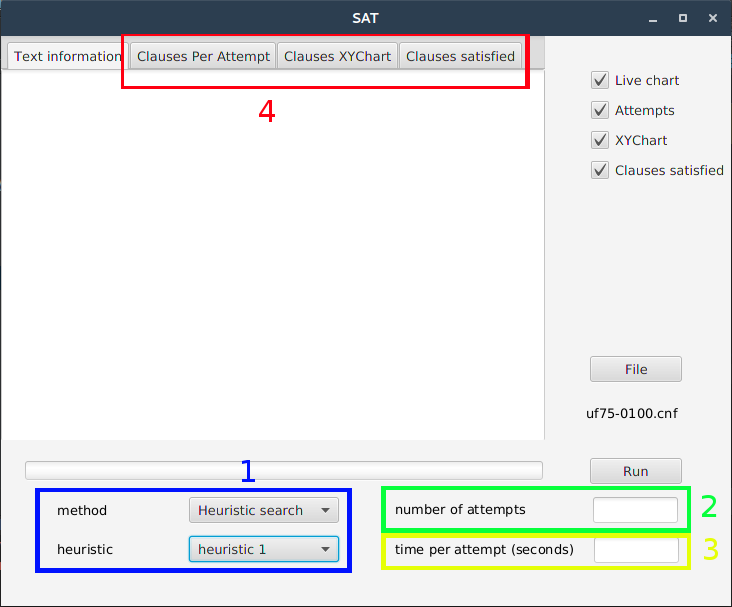
\includegraphics[width=\textwidth]{images/imgs/interface.png}
	\label{fig:mainWindow}
	\caption{Fenêtre principale }
\end{figure}
\newpage
\paragraph{Détails}
\begin{enumerate}
	\item Une liste déroulante pour choisir la méthode de recherche désirée.
	\item Le nombre de tentatives sur une même instance.
	\item La durée (en secondes) d'une tentative sur une instance.
	\item Un groupe d'onglets dédiés à l'affichage de trois types de graphiques illustratifs.
\end{enumerate}
\paragraph{}
Pour ce qu'il en est des groupes d'onglets, nous avons trois types de graphiques : 
\begin{itemize}
	\item \textbf{Attempts : } un histogramme montrant le taux de satisfiabilité pour chaque tentatives sur une instances : 
	\begin{figure}[H]\label{attemptsChart}
		\centering
		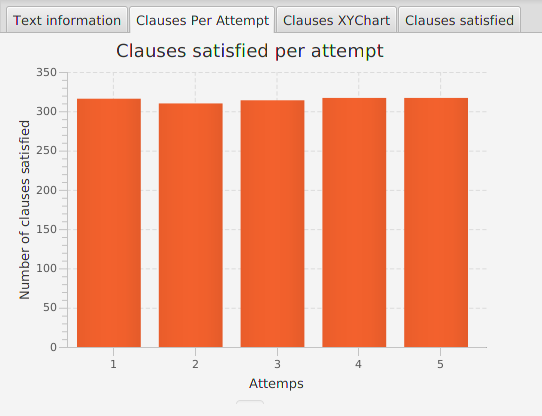
\includegraphics[scale=0.5]{images/imgs/attemptsChart.png}
		\caption{Attempts}
	\end{figure}
	\item \textbf{XYChart : } une courbe pour suivre l'évolution du taux de satisfiabilité pour chaque tentative : 
	\begin{figure}[H]\label{XYchart}
		\centering
		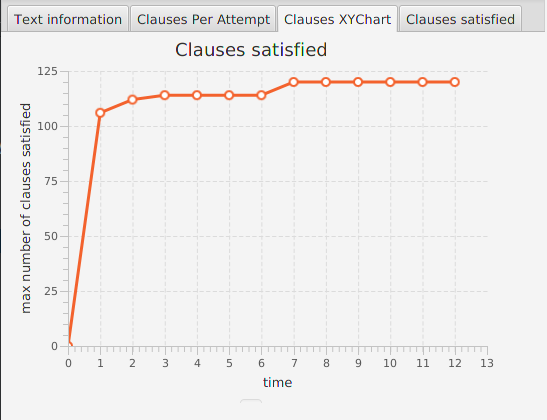
\includegraphics[scale=0.5]{images/imgs/XYChart.png}
		\caption{XYChart}
	\end{figure}
	\item \textbf{Clauses satisfied : } un histogramme qui montre la fréquence de satisfiabilité d'une clause $c_i$ durant une tentative sur l'instance courante, l'histogramme est trié pour mieux observer les données : 
	\begin{figure}[H]\label{frequencies}
		\centering
		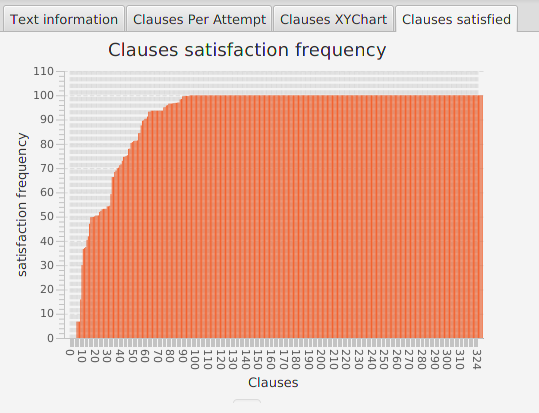
\includegraphics[scale=0.5]{images/imgs/frequenciesChart.png}
		\caption{Clauses satisfied }
	\end{figure}
\end{itemize}
\newpage
\chapter{Expérimentations}
\section{Donnés}\label{dataSet}
\paragraph{}Afin de tester notre solveur nous avons opté pour l'utilisation de fichiers benchmark qui vont représenter des instances du problème, dorénavant, et pour être plus conforme avec la terminologie du problème, nous utiliserons le terme \textbf{INSTANCE} pour désigner ces dits fichiers.
\paragraph{}
Les instances nous sont présentées sous forme de fichiers au format \textbf{DIMACS}\footnote{Représentation convetionnelle d'une instance du problème SAT}(plus de détails dans \ref{par:dimacs}) et sont disponibles en téléchargement gratuitement et librement dans \cite{Benchmark}, et sont également le fruit du travail de nombreux chercheurs dévoués.
\subsection{Format DIMACS}\label{par:dimacs}
Un fichier en format \textbf{DIMACS} est un fichier dont l'extension est \textbf{.cnf}, et est structuré de la manière suivante : \\
\begin{itemize}
	\item Le fichier peut commencer avec des commentaires, un commentaire sur une ligne commence par le caractère \textbf{'c'}
	\item La première ligne du fichier(après les commentaires) doit être structurée de la manière suivante : \textbf{\textcolor{green}{p cnf} \textcolor{blue}{nbvar} \textcolor{red}{nbclause}}
	\begin{enumerate}
		\item \textbf{\textcolor{green}{p cnf}} pour indiquer que l'instance est en forme normale conjonctive \textbf{FNC}.
		\item \textbf{\textcolor{blue}{nbvar}} indique le nombre de litéraux au total dans l'instance, à noté que chaque literal $x_{i}$ sera représenté par son indice $i$.
		\item \textbf{\textcolor{red}{nbclause}} le nombre total de clauses présentes dans l'instance.
	\end{enumerate}
	\item chaque ligne représente une conjonction de litéraux $(x_{i} \vert \lnot x_{i})$ indentifiés par un numero $i$, séparés par un blanc, avec un 0 à la fin pour marquer la fin de la ligne.
\end{itemize}
\subsection{Example}
c\\
c Un commentaire\\
c\\
c \\
p cnf 5 3\\
1 -5 4 0\\
-1 5 3 4 0\\
-3 -4 0\\
\subsection{Type d'instances}
Dans \cite{Benchmark} nous avons à notre disposition deux types d'instances pour chaque taille du problème : \\
\begin{itemize}
	\item Un ensemble d'instances satisfiable dans un fichier dénommé UF\textbf{\textcolor{blue}{XX}}-\textbf{\textcolor{red}{YY}}
	\item Un ensemble d'instances satisfiable dans un fichier dénommé UUF\textbf{\textcolor{blue}{XX}}-\textbf{\textcolor{red}{YY}}
	\item avec : 
	\begin{enumerate}
		\item \textbf{\textcolor{blue}{XX}} = nombre de litéraux
		\item \textbf{\textcolor{red}{YY}} = nombre de clauses
	\end{enumerate}
\end{itemize}
\newpage
\section{Environement de travail}
\subsection{Machines}
\paragraph{}
Pour les tests nous avons utilisé deux machines pour chaque groupes d'instances, autrement dit une machine pour effectuer les tests sur un ensembles d'instances satisfiables \textbf{\textcolor{blue}{UF75-325}}\cite{Benchmark} et une autre sur les instances contradictoires(non satisfiables) \textbf{\textcolor{red}{UUF75-325}}\cite{Benchmark}, les caractéristiques de chaque machines sont données dans les figures \ref{fig:machineA} et \ref{fig:machineB} suivantes : 
\begin{figure}[H]
	\centering
	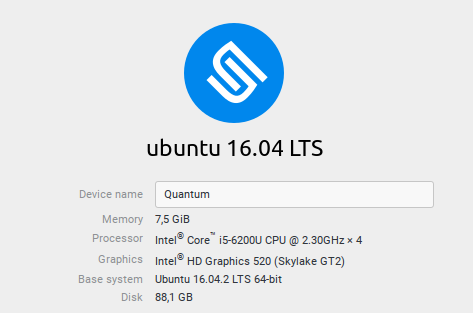
\includegraphics[scale=0.75]{images/machineWISS.png}
	\caption{Machine \textbf{A} pour les instances contradictoires}
	\label{fig:machineA}
\end{figure}
\begin{figure}[H]
	\centering
	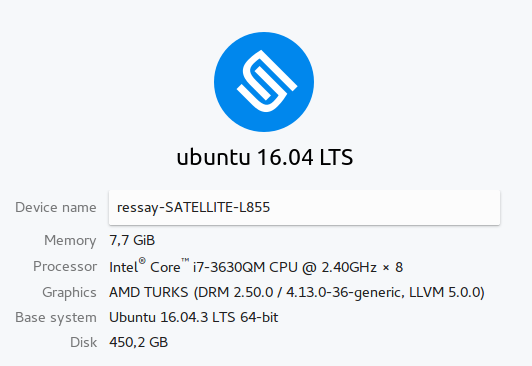
\includegraphics[scale=0.665]{images/machineYASSER.png}
	\caption{Machine \textbf{B} pour les instances satisfiables}
	\label{fig:machineB}
\end{figure}
\newpage
\subsection{Outils utilisés}
\subsubsection{Langage de programmation : }
\paragraph{}
Nous avons opté pour le langage \href{https://fr.wikipedia.org/wiki/Java_(technique)}{Java}, car il offre une grande flexibilité et un facilite l'implémentation qui est due au fait qu'il soit totallement orienté-objet.
\subsubsection{IDE : }
\paragraph{IntelliJ Idea} L'environement de dévelopement choisit est \href{https://www.jetbrains.com/idea/}{IntelliJ IDEA}, spécialement dédié au développement en utilisant le langage \href{https://fr.wikipedia.org/wiki/Java_(technique)}{Java}, il est proposé par l'entreprise \href{https://www.jetbrains.com}{JetBrains} et est caractérisé par sa forte simplicité d'utilisation et les nombreux plugins et extentions qui lui sont dédiées.

\section{Résultats}\label{tests}
\paragraph{}
Pour chacun des groupes d'instancs(i.e UF75-325 et UUF75-325) nous avons lancé les machines dédiées sur les 10 premières instances, avec 10 exécutions de durées égales à 10 mins pour chaque instance et pour chaque méthodes, les résultats sont les suivants : \\
\subsection{En largeur d'abord :}
\paragraph{}
Les résultats sont présentés d'abord sous forme de tables puis illustrés dans des histogrammes :
\paragraph{Remarque :} \label{BreadthIssueExperience} En ce qui concerne cet algorithme, nous avons eu une saturation de la mémoire après 1 min d'exécution avec la structure d'évaluation en \textbf{Bitset} (voir \ref*{def:Bitset} page \pageref{def:Bitset}) cela est principalement dû au fait que cette structure permet d'évaluer un plus grand nombre de clauses en un lapse de temps  très court là où la structure d'évaluation matrcielle ( voir \ref{def:matrix} page \pageref{def:matrix}) prend plus de temps pour faire le traitement, en conséquence le débordement de la mémoire survient mais après un temps plus conséquant, les résultats obtenus sont donc ceux observé avant le débordement.
\subsubsection{Pour les instances satisfiables :}
% Please add the following required packages to your document preamble:
% \usepackage{multirow}
\begin{table}[H]
	\centering
	\label{table:Tab_BFS_Sat}
	\begin{tabular}{|c|c|c|c|}
		\hline
		Fichiers test              & Instance & Maximum clauses & Taux  moyen de satisfiabilité \\ \hline
		\multirow{10}{*}{UF75-325} & 1        & 153             & 42,83\%                       \\ \cline{2-4} 
		& 2        & 152             & 43,94\%                       \\ \cline{2-4} 
		& 3        & 147             & 42,31\%                       \\ \cline{2-4} 
		& 4        & 140             & 42,25\%                       \\ \cline{2-4} 
		& 5        & 146             & 42,46\%                       \\ \cline{2-4} 
		& 6        & 146             & 43,05\%                       \\ \cline{2-4} 
		& 7        & 144             & 41,91\%                       \\ \cline{2-4} 
		& 8        & 160             & 44,37\%                       \\ \cline{2-4} 
		& 9        & 152             & 43,04\%                       \\ \cline{2-4} 
		& 10       & 144             & 42,58\%                       \\ \hline
	\end{tabular}
	\caption{Tableau récapitulatif des résultats pour les instances satisfiables}
\end{table}
\paragraph{}Pour mieux visualiser les données du tableau, le graphe suivant est proposé :\\

\begin{figure}[H]
	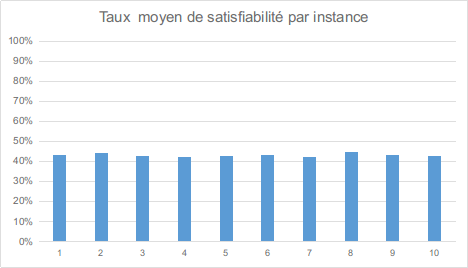
\includegraphics[width=\textwidth]{images/BFSUF75Graph.png}
	\caption{Illustration des données de \ref{table:Tab_BFS_Sat}}
\end{figure}
\newpage
\subsubsection{Pour les instances contradictoires ( non sastisfiables ) : }
% Please add the following required packages to your document preamble:
% \usepackage{multirow}
\begin{table}[H]
	\centering
	\label{table:Tab_BFS_Non_Sat}
	\begin{tabular}{|c|c|c|c|}
		\hline
		Fichiers test               & Instance & Maximum clauses & Taux moyen de satisfiabilité \\ \hline
		\multirow{10}{*}{UUF75-325} & 1        & 143             & 41,60\%                      \\ \cline{2-4} 
		& 2        & 147             & 42,95\%                      \\ \cline{2-4} 
		& 3        & 151             & 41,23\%                      \\ \cline{2-4} 
		& 4        & 136             & 41,48\%                      \\ \cline{2-4} 
		& 5        & 148             & 41,72\%                      \\ \cline{2-4} 
		& 6        & 144             & 41,05\%                      \\ \cline{2-4} 
		& 7        & 145             & 42,15\%                      \\ \cline{2-4} 
		& 8        & 145             & 41,82\%                      \\ \cline{2-4} 
		& 9        & 154             & 42,37\%                      \\ \cline{2-4} 
		& 10       & 142             & 42,15\%                      \\ \hline
	\end{tabular}
	\caption{Tableau récapitulatif des résultats pour les instances non-satisfiables}
\end{table}
\begin{figure}[H]
	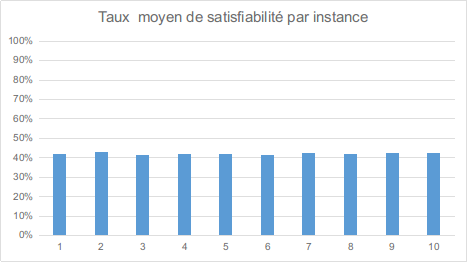
\includegraphics[width=\textwidth]{images/BFSUUF75Graph.png}
	\caption{Illustration des données de \ref{table:Tab_BFS_Non_Sat}}
\end{figure}

\newpage
\subsection{Par profondeur d'abord :}
Les résultats sont présentés d'abord sous forme de tables puis illustrés dans des histogrammes : 
\subsubsection{Pour les instances satisfiables :}
% Please add the following required packages to your document preamble:
% \usepackage{multirow}
\begin{table}[H]
	\centering
	\begin{tabular}{|c|c|c|c|}
	\hline
	Fichiers test              & Instance & Maximum clauses & Taux moyen de satisfiabilité \\ \hline
	\multirow{10}{*}{UF75-325} & 1        & 312             & 92,95\%                      \\ \cline{2-4} 
	& 2        & 306             & 92,37\%                      \\ \cline{2-4} 
	& 3        & 309             & 92,46\%                      \\ \cline{2-4} 
	& 4        & 306             & 92,65\%                      \\ \cline{2-4} 
	& 5        & 308             & 93,14\%                      \\ \cline{2-4} 
	& 6        & 310             & 94,18\%                      \\ \cline{2-4} 
	& 7        & 305             & 93,75\%                      \\ \cline{2-4} 
	& 8        & 308             & 92,49\%                      \\ \cline{2-4} 
	& 9        & 310             & 94,46\%                      \\ \cline{2-4} 
	& 10       & 306             & 94,22\%                      \\ \hline
\end{tabular}
	\caption{Tableau récapitulatif des résultats pour les instances satisfiables}
	\label{table:Tab_DFS_Sat}
\end{table}
\begin{figure}[H]
	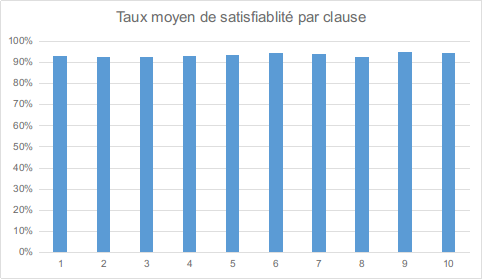
\includegraphics[width=\textwidth]{images/DFSUF75Graph.png}
	\caption{Illustration des données de la table \ref{table:Tab_DFS_Sat}}
\end{figure}


\subsubsection{Pour les instances contradictoires ( non sastisfiables ) :  }
% Please add the following required packages to your document preamble:
% \usepackage{multirow}
\begin{table}[H]
	\centering
	\begin{tabular}{|c|c|c|c|}
		\hline
		Fichiers test              & Instance & Maximum clauses & Taux moyen de satisfiabilité \\ \hline
		\multirow{10}{*}{UF75-325} & 1        & 312             & 94,37\%                      \\ \cline{2-4} 
		& 2        & 306             & 93,29\%                      \\ \cline{2-4} 
		& 3        & 309             & 94,34\%                      \\ \cline{2-4} 
		& 4        & 306             & 92,83\%                      \\ \cline{2-4} 
		& 5        & 308             & 92,61\%                      \\ \cline{2-4} 
		& 6        & 310             & 95,38\%                      \\ \cline{2-4} 
		& 7        & 305             & 92,83\%                      \\ \cline{2-4} 
		& 8        & 308             & 93,66\%                      \\ \cline{2-4} 
		& 9        & 310             & 93,60\%                      \\ \cline{2-4} 
		& 10       & 306             & 93,33\%                      \\ \hline
	\end{tabular}
	\caption{Tableau récapitulatif des résultats pour les instances non-satisfiables}
	\label{table:Tab_DFS_Non_Sat}
\end{table}
\begin{figure}[H]
	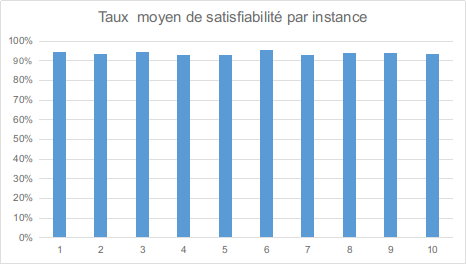
\includegraphics[width=\textwidth]{images/DFSUUF75Graph.png}
	\caption{Illustration des données de la table \ref{table:Tab_DFS_Non_Sat}}
\end{figure}
%%%%%%%%%%%%%%%%%%%%%%%%%%%%%%%%%%%%%%%%%%%%%%%%%%%%%%%%%%%%%%%%
\newpage
\subsection{Cout uniforme} :
Les résultats sont présentés d'abord sous forme de tables puis illustrés dans des histogrammes : 
\subsubsection{Pour les instances satisfiables :}
% Please add the following required packages to your document preamble:
% \usepackage{multirow}
\begin{table}[H]
	\centering
	\begin{tabular}{|c|c|c|c|}
		\hline
		Fichiers test               & Instance & Maximum clauses & Taux moyen de satisfiabilité \\ \hline
		\multirow{10}{*}{UF75-325} & 1        & 307             & 93,38\%                      \\ \cline{2-4} 
		& 2        & 304             & 93,23\%                      \\ \cline{2-4} 
		& 3        & 307             & 93,23\%                      \\ \cline{2-4} 
		& 4        & 304             & 92,77\%                      \\ \cline{2-4} 
		& 5        & 303             & 93,08\%                      \\ \cline{2-4} 
		& 6        & 302             & 92,77\%                      \\ \cline{2-4} 
		& 7        & 299             & 91,69\%                      \\ \cline{2-4} 
		& 8        & 301             & 92,00\%                      \\ \cline{2-4} 
		& 9        & 307             & 93,54\%                      \\ \cline{2-4} 
		& 10       & 305             & 93,08\%                      \\ \hline
	\end{tabular}
	\caption{Tableau récapitulatif des résultats pour les instances satisfiables}
	\label{table:Tab_UniformCost_Sat}
\end{table}
\begin{figure}[H]
	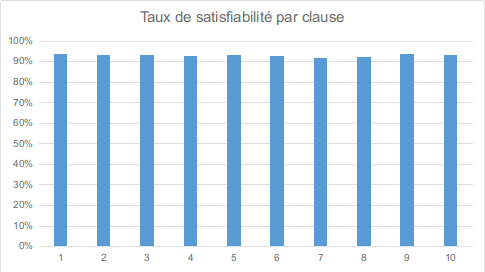
\includegraphics[width=\textwidth]{images/UniformCostUF75Graph.png}
	\caption{Illustration des données de la table \ref{table:Tab_UniformCost_Sat}}
\end{figure}


\subsubsection{Pour les instances contradictoires ( non sastisfiables ) :  }
% Please add the following required packages to your document preamble:
% \usepackage{multirow}
\begin{table}[H]
	\centering
	\begin{tabular}{|c|c|c|c|}
		\hline
		Fichiers test              & Instance & Maximum clauses & Taux moyen de satisfiabilité \\ \hline
		\multirow{10}{*}{UUF75-325} & 1        & 299             & 91,69\%                      \\ \cline{2-4} 
		& 2        & 305             & 92,77\%                      \\ \cline{2-4} 
		& 3        & 301             & 92,00\%                      \\ \cline{2-4} 
		& 4        & 307             & 94,15\%                      \\ \cline{2-4} 
		& 5        & 309             & 94,92\%                      \\ \cline{2-4} 
		& 6        & 300             & 92,00\%                      \\ \cline{2-4} 
		& 7        & 303             & 92,92\%                      \\ \cline{2-4} 
		& 8        & 301             & 92,46\%                      \\ \cline{2-4} 
		& 9        & 310             & 94,62\%                      \\ \cline{2-4} 
		& 10       & 308             & 94,42\%                      \\ \hline
	\end{tabular}
	\caption{Tableau récapitulatif des résultats pour les instances non-satisfiables}
	\label{table:Tab_UniformCost_Non_Sat}
\end{table}
\begin{figure}[H]
	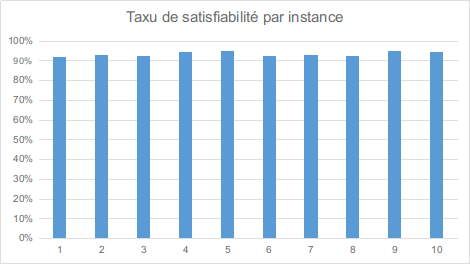
\includegraphics[width=\textwidth]{images/UniformCostUUF75Graph.png}
	\caption{Illustration des données de la table \ref{table:Tab_UniformCost_Non_Sat}}
\end{figure}

%%%%%%%%%%%%%%%%%%%%%%%%%%%%%%%%%%%%%%%%%%%%%%%%%%%%%%%%%%%%%%%%%

%%%%%%%%%%%%%%%%%%%%%%%%%%%%%%%%%%%%%%%%%%%%%%%%%%%%%%%%%%%%%%%%
\newpage
\subsection{Recherche gloutonne} :
Les résultats sont présentés d'abord sous forme de tables puis illustrés dans des histogrammes : 
\subsubsection{Pour les instances satisfiables :}
% Please add the following required packages to your document preamble:
% \usepackage{multirow}
\begin{table}[H]
	\centering
	\begin{tabular}{|c|c|c|c|}
		\hline
		Fichiers test              & Instance & Maximum clauses & Taux moyen de satisfiabilité \\ \hline
		\multirow{10}{*}{UF75-325} & 1        & 320             & 98,15\%                      \\ \cline{2-4} 
		& 2        & 319             & 97,85\%                      \\ \cline{2-4} 
		& 3        & 316             & 96,77\%                      \\ \cline{2-4} 
		& 4        & 317             & 97,23\%                      \\ \cline{2-4} 
		& 5        & 317             & 97,23\%                      \\ \cline{2-4} 
		& 6        & 317             & 97,08\%                      \\ \cline{2-4} 
		& 7        & 315             & 96,46\%                      \\ \cline{2-4} 
		& 8        & 318             & 97,23\%                      \\ \cline{2-4} 
		& 9        & 318             & 97,54\%                      \\ \cline{2-4} 
		& 10       & 316             & 97,08\%                      \\ \hline
	\end{tabular}
	\caption{Tableau récapitulatif des résultats pour les instances satisfiables}
	\label{table:Tab_Greedy_Sat}
\end{table}
\begin{figure}[H]
	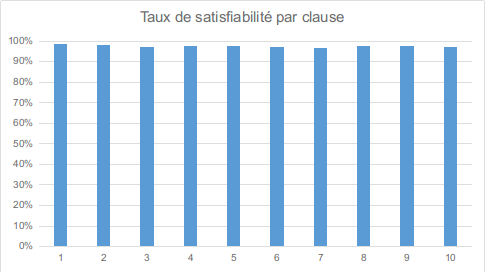
\includegraphics[width=\textwidth]{images/GreedyUF75Graph.png}
	\caption{Illustration des données de la table \ref{table:Tab_Greedy_Sat}}
\end{figure}


\subsubsection{Pour les instances contradictoires ( non sastisfiables ) :  }
% Please add the following required packages to your document preamble:
% \usepackage{multirow}
\begin{table}[H]
	\centering
	\begin{tabular}{|c|c|c|c|}
		\hline
		Fichiers test               & Instance & Maximum clauses & Taux moyen de satisfiabilité \\ \hline
		\multirow{10}{*}{UUF75-325} & 1        & 316             & 96,31\%                      \\ \cline{2-4} 
		& 2        & 315             & 96,77\%                      \\ \cline{2-4} 
		& 3        & 316             & 96,77\%                      \\ \cline{2-4} 
		& 4        & 313             & 96,31\%                      \\ \cline{2-4} 
		& 5        & 315             & 96,77\%                      \\ \cline{2-4} 
		& 6        & 311             & 95,08\%                      \\ \cline{2-4} 
		& 7        & 313             & 95,85\%                      \\ \cline{2-4} 
		& 8        & 314             & 96,00\%                      \\ \cline{2-4} 
		& 9        & 320             & 98,00\%                      \\ \cline{2-4} 
		& 10       & 310             & 94,92\%                      \\ \hline
	\end{tabular}
	\caption{Tableau récapitulatif des résultats pour les instances non-satisfiables}
	\label{table:Tab_Greedy_Non_Sat}
\end{table}
\begin{figure}[H]
	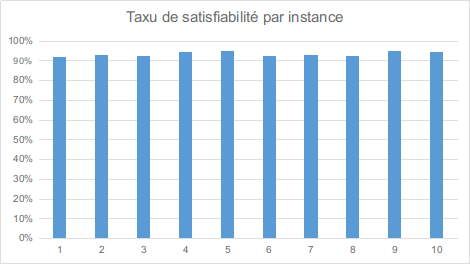
\includegraphics[width=\textwidth]{images/UniformCostUUF75Graph.png}
	\caption{Illustration des données de la table \ref{table:Tab_Greedy_Non_Sat}}
\end{figure}

%%%%%%%%%%%%%%%%%%%%%%%%%%%%%%%%%%%%%%%%%%%%%%%%%%%%%%%%%%%%%%%%%


\newpage
\subsection{Algorithme A*} :
Les résultats sont présentés d'abord sous forme de tables puis illustrés dans des histogrammes : 
\subsubsection{Pour les instances satisfiables :}
% Please add the following required packages to your document preamble:
% \usepackage{multirow}
\begin{table}[H]
	\centering
	\begin{tabular}{|c|c|c|c|}
		\hline
		Fichiers test              & Instance & Maximum clauses & Taux moyen de satisfiabilité \\ \hline
		\multirow{10}{*}{UF75-325} & 1        & 318             & 96,58\%                      \\ \cline{2-4} 
		& 2        & 318             & 97,26\%                      \\ \cline{2-4} 
		& 3        & 316             & 96,25\%                      \\ \cline{2-4} 
		& 4        & 316             & 96,31\%                      \\ \cline{2-4} 
		& 5        & 320             & 97,42\%                      \\ \cline{2-4} 
		& 6        & 320             & 97,20\%                      \\ \cline{2-4} 
		& 7        & 318             & 96,80\%                      \\ \cline{2-4} 
		& 8        & 319             & 96,83\%                      \\ \cline{2-4} 
		& 9        & 319             & 97,29\%                      \\ \cline{2-4} 
		& 10       & 319             & 97,54\%                      \\ \hline
	\end{tabular}
	\caption{Tableau récapitulatif des résultats pour les instances satisfiables}
	\label{table:Tab_Astar_Sat}
\end{table}
\begin{figure}[H]
	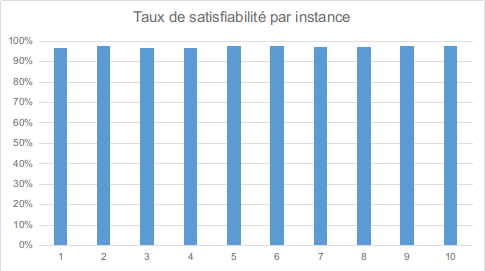
\includegraphics[width=\textwidth]{images/AstarUF75Graph.png}
	\caption{Illustration des données de la table \ref{table:Tab_Astar_Sat}}
\end{figure}


\subsubsection{Pour les instances contradictoires ( non sastisfiables ) :  }
% Please add the following required packages to your document preamble:
% \usepackage{multirow}
\begin{table}[H]
	\centering
\begin{tabular}{|c|c|c|c|}
	\hline
	Fichiers test               & Instance & Maximum clauses & Taux moyen de satisfiabilité \\ \hline
	\multirow{10}{*}{UUF75-325} & 1        & 316             & 94,65\%                      \\ \cline{2-4} 
	& 2        & 317             & 95,31\%                      \\ \cline{2-4} 
	& 3        & 315             & 94,33\%                      \\ \cline{2-4} 
	& 4        & 315             & 94,38\%                      \\ \cline{2-4} 
	& 5        & 320             & 95,47\%                      \\ \cline{2-4} 
	& 6        & 320             & 95,26\%                      \\ \cline{2-4} 
	& 7        & 317             & 94,86\%                      \\ \cline{2-4} 
	& 8        & 319             & 94,89\%                      \\ \cline{2-4} 
	& 9        & 318             & 95,34\%                      \\ \cline{2-4} 
	& 10       & 318             & 95,59\%                      \\ \hline
\end{tabular}
	\caption{Tableau récapitulatif des résultats pour les instances non-satisfiables}
	\label{table:Tab_Astar_Non_Sat}
\end{table}
\begin{figure}[H]
	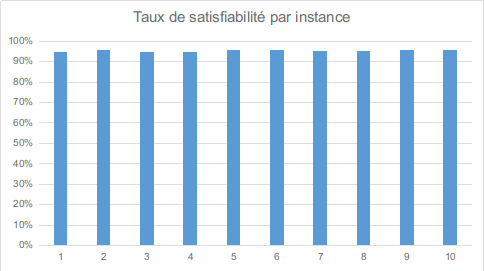
\includegraphics[width=\textwidth]{images/AstarUUF75Graph.png}
	\caption{Illustration des données de la table \ref{table:Tab_Astar_Non_Sat}}
\end{figure}
\newpage
\section{Statistiques}
\paragraph{}
Étant donné le très grand nombre de données et de résultats obtenus, nous avons décidé de récapitulé ces dérniers dans un tableau statistiques, puis dans un graphique de type \textbf{Boites-à-moustaches}

%-------------------------------------------------------------------------------
\begin{table}[H]
	\centering
	\resizebox{\textwidth}{!}{%
		\begin{tabular}{|c|c|c|c|c|c|}
			\hline
			\multicolumn{6}{|c|}{\multirow{2}{*}{UF75-325}}                                                               \\
			\multicolumn{6}{|c|}{}                                                                                        \\ \hline
			Mesure                              & BFS       & DFS       & Coût Uniforme & Recherche Gloutonne & A*        \\ \hline
			Nombre moyen de clauses satisfaites & 139,4     & 303,1     & 303,0         & 314,0               & 316,1     \\ \hline
			Taux Moyen de satisfiablié          & 42,9021\% & 93,2677\% & 93,2154\%     & 96,6000\%           &  97,2615\% \\ \hline
		\end{tabular}%
	}
	\caption{Tableau de mesures statistiques pour les instances satifsiables}
	\label{table:stat_sat}
\end{table}
\begin{figure}[H]
	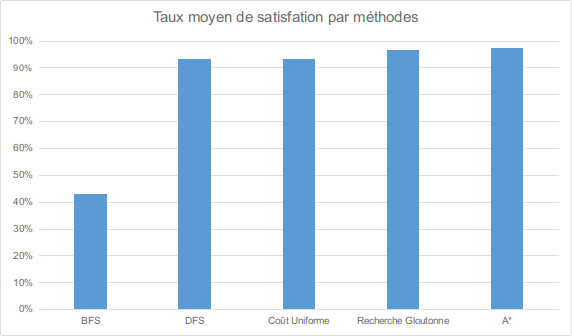
\includegraphics[width=\textwidth]{images/CompareUF75.png}
	\caption{Illustration des données de la table \ref{table:stat_sat}}
\end{figure}
\newpage
%------------------------------------------------------------------------------
\begin{table}[H]
	\centering
	
	\resizebox{\textwidth}{!}{%
		\begin{tabular}{|c|c|c|c|c|c|}
			\hline
			\multicolumn{6}{|c|}{\multirow{2}{*}{UUF75-325}}                                                               \\
			\multicolumn{6}{|c|}{}                                                                                        \\ \hline
			Mesure                              & BFS       & DFS       & Coût uniforme & Recherche gloutonne & A*        \\ \hline
			Nombre moyen de clauses satisfaites & 136,0     & 304,3     & 301,9         & 312,9               & 315,1     \\ \hline
			Taux Moyen de satisfiablié          & 41,8523\% & 93,6246\% & 92,8769\%     & 96,2769\%           & 96,9477\% \\ \hline
		\end{tabular}%
	}
	\caption{Tableau de mesures statistiques pour les instances non-satifsiables}
	\label{table:stat_non_sat}
\end{table}
%------------------------------------------------------------------------------

\begin{figure}[H]
	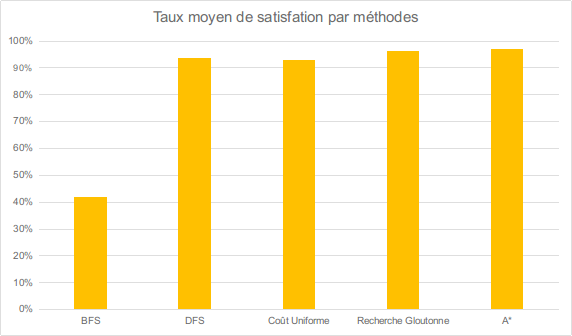
\includegraphics[width=\textwidth]{images/CompareUUF75.png}
	\caption{Illustration des données de la table \ref{table:stat_non_sat}}
\end{figure}
%------------------------------------------------------------------------------

\subsubsection{Améliorations avec BitSet}
\paragraph{}
Nous avons tenté de comparé les résultats expérimentaux en essayant différentes structures de données pour l'évaluation d'une solution et la gestion de la liste open, le tableau suivant ( voir table \ref{tab:bitsetIsLayfu} )  \ démontre que la structure du BitSet proposée évalue 15 à 190 fois ( selon la géstion de open ) plus de clauses en une seconde que la struture de matrice, combiner cette représentation avec une gesion en tas de open, nous a fait gagné un temps assez important lors de l'évaluation et le réarrangement de open.
\begin{center}\label{tab:bitsetIsLayfu}
	\begin{tabular}{|c | c| c|}
		\hline
		\backslashbox{gestion de open}{évaluation par}& Matrice & Bitset\\\hline
		liste triée& 205124 éval/s& 11952330 éval/s\\\hline
		tas & 237532 éval/s & 37252319 éval/s\\\hline
		FIFO & 238403 éval/s & 3149722 éval/s\\\hline
		LIFO & 213397 éval/s& 40879427 éval/s\\\hline
		\end{tabular}
		\captionof{table}{Nombre d'évaluations par seconde} 
\end{center}
		
		
		
\section{Comparaison entres les cinq méthodes}
\paragraph{}
Pour conclure ce chapitre, nous allons mainetant comparer les différentes méthodes selon la rapidité d'exécution, l'espace mémoire utilisé et le taux de satisfiabilité enregistré.
\paragraph{}
Nous avons remarqué à travers les nombreux tests que les deux catégories de stratégies de recherche avaient des forces et des lacunes, pour citer des exemples, la recherche par profondeur d'abord et en largeur d'abord de part sa simplicité, sont de bonnes stratégies de recherche, mais dont les limites sont vites atteintes, la première est certe peu gourmande en espace mémoire, mais ne trouve pas la solution en un temps assez rapide, la deuxième quant à elle nous garantie (si le coût pour passer d'un noeud à un autre est le même quelques soient les noeuds choisis) de trouver la solution avec le plus petit nombre de litéraux possible, mais en contre partie consomme énormemment de mémoire, ce qui peut conduire à un débordement de la mémoire très rapidement\label{BreadthIssueCompare}.
\paragraph{}
Pour ce qu'il en est de l'agrotithme de recherche par coût uniforme, il se voit être un compromis entre l'agorithme DFS\footnote{Depth first search} (voir \ref{DFSdef}) et l'algorithme BFS(\footnote{Breadth first search} (voir \ref{BFSdef}, il assure de trouver la solution avec un potentiel débordement de mémoire, mais peut aussi prendre un temps exponentiel pour trouver la solution (\ref{DijkstraDef}), les expérimentations réalisés en sont la preuve.
\paragraph{}
Quand on bascule vers la deuxième catégorie, on se rend vite commpte que l'ajout d'une heuristique peut réduire le temps de recherche d'une façon significative, ce que fait l'algorithme DFS en 10-15 mins peut être fait en quelques secondes avec l'algorithme de recherches gloutonne ou bien A*, cependant le gain en rapidité ne masque pas le fait que l'espace mémoire reste aussi soumis à un débordement ( moins fréquemment mais ça reste un risque potentiel), de plus la difficulté de trouver de bonnes heuristiques ( admissibles par exemple ) demeure un challenge du point de vue théorique et pratique, à noté aussi que très souvent, l'algorithme A* se limite à une recherche dans un maximum local, ce qui peut ralentir le processus de recherche de solutions optimales.
\paragraph{}
Une remarque à faire concernant l'ensemble des méthodes utilisées est que les résultats, malgré le fait que le choix des noeuds soit àléatoire, ne diffèrent pas d'une exécution à une autre sur une même instance ( pour A* par exemple on est dans les 96\%-97\% de taux de satisfiabilité sur les benchmarks fournis) , cela est dû principalement au fait que les fréquences d'apparitions des litéraux soient très proches les unes des autres, aisni choisir un litéral (ou sa négation) plutôt qu'un autre n'influe pas vraiment sur le résultat final.
\newpage
\chapter*{Conclusion}
\paragraph{}
En conclusion de ce travail, nous pouvons dire malgré la simplicité apparente d'un problème, il est très souvent impossible de le résoudre à l'aide de méthodes dites \textbf{classiques}, il est vrai qu'un taux de réussite de 97\% par exemple peut paraître suffisait, on ne doit pas oublié que ce taux évolue selon la taille du problème, en effet sur les instances de tailles moyenne vue dans cette partie du tp, il aurait été préférable de trouver des méthodes qui avoisinent les 99\% de taux de réussite, mais il est évident que ces méthodes représentent les limites des méthodes classiques, c'est ainsi de façon naturelle et sensée, que nous allons passé des méthodes heuristiques aux méta-heuristiques, une évolution nécessaire pour ne serait ce qu'approximer de façon plausibles et suffisante la solution optimale cachée derrière cet océan de solutions.
%%%%%%%
%%Include Part 2
\part{Approche par espace des solutions BSO}

\chapter{Introduction : }
	\section{Problématique : }
	\paragraph{Limite des méthodes de recherche CLASSIQUES}
	\section{Définitions}
		\subsection{Espace des solutions}
		\paragraph{}
		
		\subsection{Metaheuristique}
		\paragraph{}
		\subsection{Intelligence en essaim (Swarm intelligence) }
		\paragraph{}
		\subsection{Bee swarm optimization (BSO)}
		\paragraph{} 
\chapter{Implémentation de l'algorithme BSO pour le problème SAT}
	\section{Structures de données}
	\subsection{Représentation des solutions}
	\subsection{}
%%Amaze me here bro

\chapter{Expérimentations}
	\section{Données}
	\paragraph{}
	%%Basically same shit as before
	\section{Résultats}
	\paragraph{}
		\subsection{Pour les instances satisfiables}
		\paragraph{}
		%We choose the 3 best sets of parameters here
		%We plot the results
		\subsection{Pour les instances non satisfiables}
		\paragraph{}
		%We choose the 3 best sets of parameters here
		%We plot the results
	\section{Comparaison avec les méthodes de \ref{part1}}
	\paragraph{}
	%talk about how BSO is amazing

\part{Approche par espace des solutions ACO}

\chapter{Introduction : }
\section{Problématique : }
\paragraph{Limite de BSO }
Bien l'algorithme BSO (voir \ref{part2})présente des résultats très satisfaisants, il a cependant quelques points faibles qui sont liés à la recherche des bonnes valeurs des paramètres empiriques , l'ajustement dynamique a permit de palier a ce problème, mais il reste aussi l'aspect stochastique aléatoire très imprévisible des méta-heuristiques, c'est là qu'entre en scène une nouvelle familles de  M.H\footnote{Méta-heuristique} appelées ACO (\textbf{Ant Colony Optimization}) pour essayer de marier méthode constructive et méthode évolutionnaire.
\section{Définitions}
\subsection{Ant Colony Optimization(ACO)}
\paragraph{}
Les algorithmes de colonies de fourmis sont des algorithmes inspirés du comportement des fourmis, et qui constituent une famille de métaheuristiques d’optimisation principalement conçues pour des problèmes de \textbf{path-finding}\footnote{Problème visant a trouver le chemin le plus court d'un point de départ A à un point d'arrivée B}.
Dans cette partie du projet nous allons nous intéresser à deux implémentation d'une M.H ACO, à savoir \textbf{AS}(Ant System) et \textbf{ACS}(Ant Colony System).
\begin{figure}[H]
	\centering
	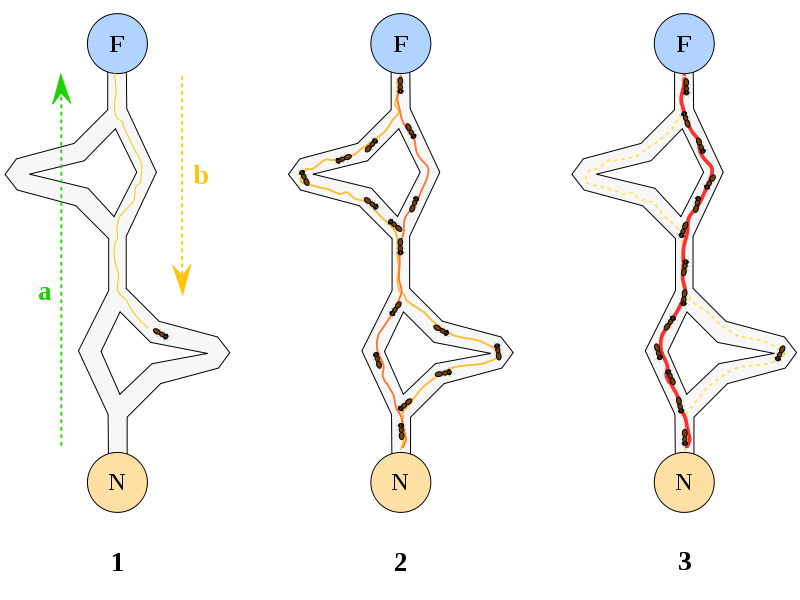
\includegraphics[scale=0.25]{images/ants.png}
	\caption{Abeilles communiquant pour la recherche de nourriture}
\end{figure}

\subsubsection{Ant System(AS)}
\paragraph{}\label{AS}
Cette variante d'ACO fut l'une des première a être développée, elle se base sur une approche probabiliste du choix du chemin a parcourir par la fourmille, en effet une fourmille en temps normal réagit à un stimulus naturel qui la \textbf{Phéromone}, une fourmille suivra instinctivement la trace de phéromones la plus forte la plus part du temps trace précédente.

\subsubsection{Ant Colony System(ACS)}
\paragraph{}\label{ACS}
Pensé comme une amélioration d'\textbf{AS}, ACS permet une modélisation plus fidèle à la vie réelle en introduisant les principes suivants: 
\begin{itemize}
	\item La mise a jour de la trace de phéromones enligne(effectuée par chaque fourmille lors de son passage sur un état) et hors-ligne(effectué à la fin de la construction de toutes les solutions des fourmilles)
	\item La marche aléatoire(RandomWalk\footnote{Modèle mathématique  d'un système possédant une évolution composée d'une succession de pas aléatoires, ou effectués « au hasard ».}) qui servira de règle de transition pour aller d'un état à un autre.
	\item Exploitation, c'est le fait de suivre la trace de phéromones la plus forte( le stimulus le plus fort).
	\item Exploration, c'est le fait de prendre l'initiative d'explorer de nouveaux états sans pour autant tenir compte de la trace de phéromones la plus forte
\end{itemize}


\subsection{Phéromones}
Pour finir il nous faut introduire le concept de la phéromone. Dans la nature, la phéromone es une molécule chimique produite par un organisme, qui induit un comportement spécifique chez un autre membre de la même espèce, dans notre cadre de la recherche de solutions optimales pour une problème donnée, elle peut être perçu comme une valeur numérique attaché un état de la solution(cela reste une interprétation générale qui peut varier selon le problème).



%Add it to implementation :
%, et déposera ensuite une petite quantité de cette phéromone sur son passage. quand toutes les fourmilles finissent de construire leur solution, une mise a jour des traces de phéromones est activée et cela selon la quantité déjà présente dans la
\chapter{Implémentation des algorithmes AS/ACS pour le problème SAT}
	\section{Structures de données:}
	\paragraph{}
	Vu les très bonnes performance réalisée par les structures de donnée vues dans \ref{part1}, nous avons logiquement opté pour les même représentations pour l'implémentation d'AS/ACS, à savoir : 
	\subsection{Représentation d’instance et de solutions SAT:}
	\paragraph{}
	\begin{flalign*}
	x_{1} \lor \neg x_{2} \lor x_{4} \\
	\neg x_{2} \lor x_{3} \lor x_{4} \\
	\neg x_{1} \lor x_{2} \lor \neg x_{3}
	\end{flalign*}
	Et la solution suivante:\\
	\begin{center}
		$x_{1} \leftarrow true$, $x_{2} \leftarrow false$, $x_{3} \leftarrow true$, $x_{4} \leftarrow false $
	\end{center}
	
	La représentation:\\
	
	\definecolor{green}{rgb}{0.5,1,0.5}
	\begin{center}
		\begin{tabular}{|c | c| c| c| c|}
			\hline
			$x_{1}$& $x_{2}$ &$x_{3}$ &$x_{4}$ \\\hline
			1 & 0 & 1 & 0 \\\hline
		\end{tabular}\\
		Solution
	\end{center}
	\begin{minipage}{0.5\textwidth}
		\centering
		\begin{tabular}{|c | c| c| c|}
			\hline
			\rowcolor{green}
			$x_{1}$& 1 & 0 & 0 \\\hline
			$x_{2}$& 0 & 0 & 1 \\\hline
			\rowcolor{green}
			$x_{3}$& 0 & 1 & 0 \\\hline
			$x_{4}$& 1 & 1 & 0 \\\hline
		\end{tabular}
	\end{minipage}
	\hfillx
	\begin{minipage}{0.5\textwidth}
		\centering
		\begin{tabular}{|c | c| c| c|}
			\hline
			$\neg x_{1}$& 0 & 0 & 1 \\\hline
			\rowcolor{green}
			$\neg x_{2}$& 1 & 1 & 0 \\\hline
			$\neg x_{3}$& 0 & 0 & 1 \\\hline
			\rowcolor{green}
			$\neg x_{4}$& 0 & 0 & 0 \\\hline
		\end{tabular}
	\end{minipage}\\
	\begin{center}
		Instance
	\end{center}
	On peut calculer les clauses satisfaites par la solution en utilisant le or logique entre les Bitset de ses littéraux:
	\begin{center}
		\begin{minipage}{0.5\textwidth}
			\centering
			\begin{tabular}{| c| c| c|c|}
				\hline
				$x_{1}$& 1 & 0 & 0 \\\hline
			\end{tabular}
		\end{minipage}
		\\~\\
		OR
		\\~\\
		\begin{minipage}{0.5\textwidth}
			\centering
			\begin{tabular}{|c | c| c| c|}
				\hline
				$x_{3}$& 0 & 1 & 0 \\\hline
			\end{tabular}
		\end{minipage}
		\\~\\
		OR
		\\~\\
		\begin{minipage}{0.5\textwidth}
			\centering
			\begin{tabular}{| c| c| c|c|}
				\hline
				$\neg x_{2}$& 1 & 1 & 0 \\\hline
			\end{tabular}
		\end{minipage}
		\\~\\
		OR
		\\~\\
		\begin{minipage}{0.5\textwidth}
			\centering
			\begin{tabular}{|c | c| c| c|}
				\hline
				$\neg x_{4}$& 0 & 0 & 0 \\\hline
			\end{tabular}
		\end{minipage}
		\begin{center}
			
			$\downarrow$
			\\~\\
			\begin{tabular}{|c | c| c| c|}
				\hline
				$Bitset$ résultat& 1 & 1 & 0 \\\hline
			\end{tabular}
		\end{center}
	\end{center}
	
	
	\subsection{La table des Phéromones}
	\paragraph{}
	La différence entre BSO et ACO réside dans le fait qu'une solution n'est pas obtenue selon le voisinage d'une autre solution, mais est construite pas à pas selon une règle de transition d'un état à un autre. Pour garder trace des phéromones déposées par les fourmilles lors de la construction de leur solutions respectives, nous pouvons utilisée un tableau a deux dimensions(Matrice) dont les lignes sont les variables de la solution, et les colonnes les deux litéraux de la variable associée. le schéma suivant traduit cela : 
	
	\begin{minipage}{\textwidth}
		\centering
		\begin{table}[H]
			\centering
			\begin{tabular}{|c|c|c|}
				\hline
				$i$ & $x_{i}$ & $\lnot x_{i}$ \\ \hline
				1   & 0.1     & 0.1           \\ \hline
				2   & 0.1     & 0.1           \\ \hline
				3   & 0.1     & 0.1           \\ \hline
				4   & 0.1     & 0.1           \\ \hline
			\end{tabular}
			\caption{Table des phéromones initiale}
		\end{table}
		$\Downarrow$
		\begin{table}[H]
			\centering
			\begin{tabular}{|c|c|c|}
				\hline
				$i$ & $x_{i}$ & $\lnot x_{i}$ \\ \hline
				1   & 0.1     & 0.1           \\ \hline
				2   & 0.1     & 0.1           \\ \hline
				3   & 0.1     & 0.1           \\ \hline
				4   & 0.325     & 0.102           \\ \hline
			\end{tabular}
			\caption{Table des phéromones après le passage d'une fourmille}
		\end{table}
	\end{minipage}
	\\~\\
	La figure illustre le processus de dépôt de phéromones, celui de l'évaporation sera vu plus tard car il dépend du choix de l'algorithme dérivant d'ACO(i.e soi AS ou bien ACS).
	\section{Conception et pseudo-code:}
	\paragraph{}
	L'algorithme ACO a une structure de base très simple, elle se résume à l'algorithme suivant : 
	\begin{algorithm}
		\SetAlgoLined
		\KwResult{retourne la meilleure solution trouvée}
		\textbf{init}($pheromons$)\;
		\textbf{init}($allParameters$)
		$meilleureSolution \gets randomSolution$\;
		\While{$\neg$\textbf{fin()}}{
			\ForEach{$fourmille \in fourmilles$}
			{
				\textbf{contruireSolution($fourmille$)}\;
				\If{$isValide(fourmille.solution)$ }{
					\Return $fourmille.solution$\;
				}
			}
			\textbf{postConstructionActions($fourmilles$)}\;
			\tcp{sera vu plus en détails dans AS/ACS}\;
			\If{\textbf{bestSolution}($fourmilles$)>$meilleureSolution$}{
					$meilleureSolution \gets$ \textbf{bestSolution($fourmilles$)}\;		
				}
				\textbf{miseAjourt}($pheromons$)\;
			}
		\Return $meilleureSolution$\;
		\caption{Algorithme de recherche ACO}
	\end{algorithm}\\
	\newpage
	\paragraph{}
	Maintenant que nous avons vu le principale fonctionnement d'ACO, il est temps de spécifier le comportement d'AS et ACS:
	\subsection{AS(Ant System)}
	Il repose comme cité dans \ref{AS} sur une règle de transition probabiliste que l'on va détailler après avoir montré le pseudo code suivant : 
	
	\begin{algorithm}[H]
		\SetAlgoLined
		\KwResult{retourne la meilleure solution trouvée}
		\textbf{init}($pheromons$)\;
		\textbf{init}($allParameters$)
		$meilleureSolution \gets randomSolution$\;
		\lFor{$t=1$ \KwTo maxItter}{
			\ForEach{$fourmille \in fourmilles$}
			{
				\Repeat{$fourmille$ construit sa solution}
				{
					$P_{i,j} \gets$ \textbf{calculerProba()}\;
					$nextState \gets $ \textbf{selectNextBy($P_{i,j}$)}\; 
				}
				$evaluation$ = \textbf{evaluer($fourmlle.solution$)}\;
				\If{$evaluation$ = $bestScore$}{
					\Return $fourmille.solution$\;
				}
				\textbf{onlinePheromonsUpdate($pheromons$)}\;
			}
			\If{\textbf{bestSolution}($fourmilles$)>$meilleureSolution$}{
				$meilleureSolution \gets$ \textbf{bestSolution($fourmilles$)}\;		
			}
			
		}
		\Return $meilleureSolution$\;
		\caption{Algorithme de recherche AS}
	\end{algorithm}
	
	\paragraph{}Nous allons maintenant détailler l'algorithme : 
	\begin{enumerate}
		\item Ligne 1-2 : initialiser les paramètres empiriques et la table des phéromones a une valeur très petite arbitraire(0.1 par exemple).
		\item Ligne 5 : calculer la probabilité du litéral $j$ de la variable $i$ selon la formule suivante : \\
		\begin{equation}
			P_{i,j} = \frac{\lbrack T_{i,j} \rbrack^{\alpha}* \lbrack\mu_{i,j}\rbrack^{\beta}}{\sum\limits_{lit \in Literals}{\lbrack T_{i,lit} \rbrack^{\alpha}* \lbrack\mu_{i,lit}\rbrack^{\beta}}}
		\end{equation}
		Autrement dit : le literal $x_{i}$ (réspec. $\lnot x_{i}$) aura une probabilité $P_{x_{i}}$ (respec. $P_{\lnot x_{i}}$ ) d'être choisi comme prochain état de la solution en cours de construction.
		
		\item Ligne 6 : pour simuler un processus aléatoire, il suffit de tirer au hasard un nombre aléatoire $q$, si $q < P_{x_{i}}$ alors le prochain literal à être choisis sera $x_i$, sinon ce sera $\lnot x_i$ ( on prend la densité de probabilités la plus proche du nombre aléatoire $q$ )
		
		
		\item Ligne 12 : la mise a jour en-ligne de la table de phéromones se fait selon la formule suivante : 
		\begin{eqnarray}
			P_{i,j} = (1-\rho)T_{i,j} + \rho \sum_{a \in Ants}{\Delta_a T_{i,j}}
		\end{eqnarray}
		\newpage
		oû : 
		\begin{itemize}
			\item $\rho$ est le taux d'évaporation de la phéromone
			\item $\Delta_a T_{i,j}$ est le taux de phéromones ajouté par la fourmille $a$ sur le litéral $j$ de la variable $x_i$
			dans notre cas nous avons prit : \\
			\begin{equation}
				\Delta_a T_{i,j} = nbrClauseSatisfaites(x_{i,j})/nbrClauseTotal
			\end{equation}
			le but étant de déposer un taux de phéromones plus élevé si le literal nous rapproche(en théorie) de la solution positive.
		\end{itemize}
	\end{enumerate}
	
	\paragraph{}
	le processus de construction à un instant $t$ est illustré comme suit : 
	
	\begin{minipage}{0.5\textwidth}
		\begin{table}[H]
			\centering
			\label{my-label}
			\begin{tabular}{|c|}
				\hline
				\begin{tabular}[c]{@{}c@{}}.\\ .\\ .\end{tabular} \\ \hline
				1                                                 \\ \hline
				0                                                 \\ \hline
				0                                                 \\ \hline
				?                                                 \\ \hline
			\end{tabular}
		\end{table}
		\centering
		$\downarrow$
	\end{minipage}
	\begin{minipage}{0.5\textwidth}
		\begin{table}[H]
			\centering
			\begin{tabular}{|c|c|}
				\hline
				\begin{tabular}[c]{@{}c@{}}.\\ .\\ .\end{tabular} & \begin{tabular}[c]{@{}c@{}}.\\ .\\ .\end{tabular} \\ \hline
				\rowcolor[HTML]{9AFF99} 
				0.254                                             & \cellcolor[HTML]{FD6864}0.154                     \\ \hline
				\rowcolor[HTML]{FD6864} 
				0.001                                             & \cellcolor[HTML]{67FD9A}0.155                     \\ \hline
				\rowcolor[HTML]{FD6864} 
				0.1                                               & \cellcolor[HTML]{67FD9A}0.512                     \\ \hline
				\rowcolor[HTML]{67FD9A} 
				0.244                                             & \cellcolor[HTML]{FD6864}0.2                      \\ \hline
			\end{tabular}
		\end{table}
		\centering
		$\downarrow$
	\end{minipage}
	
	
	
	
	\begin{minipage}{0.5\textwidth}
		\begin{table}[H]
			\centering
			\label{my-label}
			\begin{tabular}{|c|}
				\hline
				\begin{tabular}[c]{@{}c@{}}.\\ .\\ .\end{tabular} \\ \hline
				1                                                 \\ \hline
				0                                                 \\ \hline
				0                                                 \\ \hline
				1                                                 \\ \hline
			\end{tabular}
		\end{table}
	\end{minipage}
	\begin{minipage}{0.5\textwidth}
		\begin{table}[H]
			\centering
			\begin{tabular}{|c|c|}
				\hline
				\begin{tabular}[c]{@{}c@{}}.\\ .\\ .\end{tabular} & \begin{tabular}[c]{@{}c@{}}.\\ .\\ .\end{tabular} \\ \hline
				\rowcolor[HTML]{9AFF99} 
				0.254                                             & \cellcolor[HTML]{FD6864}0.154                     \\ \hline
				\rowcolor[HTML]{FD6864} 
				0.001                                             & \cellcolor[HTML]{67FD9A}0.155                     \\ \hline
				\rowcolor[HTML]{FD6864} 
				0.1                                               & \cellcolor[HTML]{67FD9A}0.512                     \\ \hline
				\rowcolor[HTML]{67FD9A} 
				0.244 + 0.2                                             & \cellcolor[HTML]{FD6864}0.2+0.05                      \\ \hline
			\end{tabular}
		\end{table}
	\end{minipage}
	\paragraph{}
	Nous pouvons noter que ce comportement n'est pas toujours représentatif de la réalité, en effet selon cet algorithme la fourmille ne fait qu'explorer bêtement les traces de phéromones, il serait intéressant de modéliser le phénomènes d'exploitation de la plus forte trace de phéromone, cela a été introduit grâce à l'algorithme ACS. 
	\newpage
	\subsection{ACS(Ant Colony System)}
	Comme cité dans \ref{ACS}, ACS est une amélioration de AS dans le sens ou une fourmille peut adopter une comportement aléatoire lors de l'application de la règle de transition, elle pourra soit explorer de nouvelles opportunités ou bien exploiter la meilleure trace à sa disposition, la fourmille n'étant pas doté d'une intelligence assez développé pour faire ce choix systématique, elle choisira selon l'instant donné totalement au hasard, bien sur ce choix est conditionné par le fait que la plus part du temps une fourmille choisira la trace de phéromones la plus forte instinctivement. ACS se démarque aussi par l'ajout d'une mise a jour hors-ligne de la table des phéromones lorsque toute les fourmilles auront finit la construction de leurs solutions, le principe est que la fourmille ayant fournit la meilleure solution ajoute la quantité de phéromone proportionnelle à sa solution, en gardant aussi la mise à jour en-ligne(step by step ) des fourmilles lors  de la construction de leurs solutions respectives.
	
	
	\begin{algorithm}[H]
		\SetAlgoLined
		\KwResult{retourne la meilleure solution trouvée}
		\textbf{init}($pheromons$)\;
		\textbf{init}($allParameters$)
		$meilleureSolution \gets randomSolution$\;
		\lFor{$t=1$ \KwTo maxItter}{
			\ForEach{$fourmille \in fourmilles$}
			{
				\Repeat{$fourmille$ construit sa solution}
				{
					$P_{i,j} \gets$ \textbf{calculerProba()}\;
					$nextState \gets $ \textbf{selectNextBy($P_{i,j}$)}\; 
				}
				$evaluation$ = \textbf{evaluer($fourmlle.solution$)}\;
				\If{$evaluation$ = $bestScore$}{
					\Return $fourmille.solution$\;
				}
				\textbf{onlinePheromonsUpdate($pheromons$)}\;
			}
			\If{\textbf{bestSolution}($fourmilles$)>$meilleureSolution$}{
				$meilleureSolution \gets$ \textbf{bestSolution($fourmilles$)}\;		
			}
			\textbf{offLinePheromonsUpdate($pheromons,meilleurFourmille$)}\;
			
			
		}
		\Return $meilleureSolution$\;
		\caption{Algorithme de recherche ACS}
	\end{algorithm}
	
	
	\begin{enumerate}
		\item Ligne 1-2 : initialiser les paramètres empiriques et la table des phéromones a une valeur très petite arbitraire(0.1 par exemple).
		\item Ligne 5 : calculer la probabilité du litéral $j$ de la variable $i$ selon la formule suivante : \\
		\begin{equation}
		P_{i,j} = \frac{\lbrack T_{i,j} \rbrack^{\alpha}* \lbrack\mu_{i,j}\rbrack^{\beta}}{\sum\limits_{lit \in Literals}{\lbrack T_{i,lit} \rbrack^{\alpha}* \lbrack\mu_{i,lit}\rbrack^{\beta}}}
		\end{equation}
		Autrement dit : le literal $x_{i}$ (réspec. $\lnot x_{i}$) aura une probabilité $P_{x_{i}}$ (respec. $P_{\lnot x_{i}}$ ) d'être choisi comme prochain état de la solution en cours de construction.
		
		\item Ligne 6 : pour simuler un processus de la marche aléatoire, on tire au hasard un nombre $q$, si $q<q_0$ alors on choisit le literal avec la combinaison \textbf{pheromone|heuristique} maximale, sinon si $q < P_{x_{i}}$ alors le prochain literal à être choisis sera $x_i$, sinon ce sera $\lnot x_i$ ( on prend la densité de probabilités la plus proche du nombre aléatoire $q$ ).\\
		plus formellement on a :
			 
			 
			\begin{equation*}
				\text{si }q \leq q_0 \\
			\end{equation*}
			\\
			\[   
			P_{i,j} = 
			\begin{cases}
			1 & \quad\text{si $i =$}argmax\lbrace\lbrack T_{i,j} \rbrack^{\alpha}* \lbrack\mu_{i,j}\rbrack^{\beta}\rbrace \\\\
			0 & \quad\text{sinon}\\
			\end{cases}
			\]
			
			\begin{equation*}
			\text{si } q > q_0 \\
			\end{equation*}
			\\
			\begin{equation*}
				P_{i,j} = 
				\frac{\lbrack T_{i,j} \rbrack^{\alpha}* \lbrack\mu_{i,j}\rbrack^{\beta}}{\sum\limits_{lit \in Literals}{\lbrack T_{i,lit} \rbrack^{\alpha}* \lbrack\mu_{i,lit}\rbrack^{\beta}}}
			\end{equation*}
			
			
		
		
		
		\item Ligne 12 : la mise a jour en-ligne de la table de phéromones se fait selon la formule suivante : 
		\begin{eqnarray}
		P_{i,j} = (1-\rho)T_{i,j} + \rho \tau_0
		\end{eqnarray}
		oû : 
		$\tau_0$ est le taux de phéromones initial
		\item Ligne 17 : la mise à jour offline de la table des phéromones est réalisée de la manière suivante : 
		\begin{equation*}
			P_{i,j} = (1-\rho)T_{i,j} + \rho \Delta T_{i,j}^{bestAnt}
		\end{equation*}
		\begin{itemize}
			\item $\rho$ est le taux d'évaporation de la phéromone
			\item $\Delta_a T_{i,j}$ est le taux de phéromones ajouté par la fourmille $a$ sur le litéral $j$ de la variable $x_i$
			dans notre cas nous avons prit : \\
			\begin{equation}
			\Delta T{i,j}^{bestAnt} = nbrClauseSatisfaites(x_{i,j}^{bestAnt})/nbrClauseTotal
			\end{equation}
			l'idée est que la fourmille avec le plus haut taux de réussite dépose plus de phéromones après la construction des solutions.
		\end{itemize}
	\end{enumerate}
	\newpage
	\paragraph{}
	le schéma suivant aide à mieux comprendre : \\
	\begin{minipage}{0.5\textwidth}
		\begin{table}[H]
			\centering
			\label{my-label}
			\begin{tabular}{|c|}
				\hline
				\begin{tabular}[c]{@{}c@{}}.\\ .\\ .\end{tabular} \\ \hline
				1                                                 \\ \hline
				0                                                 \\ \hline
				0                                                 \\ \hline
				?                                                 \\ \hline
			\end{tabular}
		\end{table}
		\centering
		$\downarrow$
	\end{minipage}
	\begin{minipage}{0.5\textwidth}
		\begin{table}[H]
			\centering
			\begin{tabular}{|c|c|}
				\hline
				\begin{tabular}[c]{@{}c@{}}.\\ .\\ .\end{tabular} & \begin{tabular}[c]{@{}c@{}}.\\ .\\ .\end{tabular} \\ \hline
				\rowcolor[HTML]{9AFF99} 
				0.254                                             & \cellcolor[HTML]{FD6864}0.154                     \\ \hline
				\rowcolor[HTML]{FD6864} 
				0.001                                             & \cellcolor[HTML]{67FD9A}0.155                     \\ \hline
				\rowcolor[HTML]{FD6864} 
				0.1                                               & \cellcolor[HTML]{67FD9A}0.512                     \\ \hline
				\rowcolor[HTML]{67FD9A} 
				0.244                                             & \cellcolor[HTML]{FD6864}0.2                      \\ \hline
			\end{tabular}
		\end{table}
		\centering
		$\downarrow$
	\end{minipage}
	
	
	
	
	\begin{minipage}{0.5\textwidth}
		\begin{table}[H]
			\centering
			\label{my-label}
			\begin{tabular}{|c|}
				\hline
				\begin{tabular}[c]{@{}c@{}}.\\ .\\ .\end{tabular} \\ \hline
				1                                                 \\ \hline
				0                                                 \\ \hline
				0                                                 \\ \hline
				1                                                 \\ \hline
			\end{tabular}
		\end{table}
	\end{minipage}
	\begin{minipage}{0.5\textwidth}
		\begin{table}[H]
			\centering
			\begin{tabular}{|c|c|}
				\hline
				\begin{tabular}[c]{@{}c@{}}.\\ .\\ .\end{tabular} & \begin{tabular}[c]{@{}c@{}}.\\ .\\ .\end{tabular} \\ \hline
				\rowcolor[HTML]{9AFF99} 
				0.254                                             & \cellcolor[HTML]{FD6864}0.154                     \\ \hline
				\rowcolor[HTML]{FD6864} 
				0.001                                             & \cellcolor[HTML]{67FD9A}0.155                     \\ \hline
				\rowcolor[HTML]{FD6864} 
				0.1                                               & \cellcolor[HTML]{67FD9A}0.512                     \\ \hline
				\rowcolor[HTML]{67FD9A} 
				0.244 + 0.1                                             & \cellcolor[HTML]{FD6864}0.2+0.1                      \\ \hline
			\end{tabular}
		\end{table}
	\end{minipage}
	\begin{minipage}{\textwidth}
		~~\\\\
		\centering
		$\downarrow$
		\begin{table}[H]
			\centering
			\begin{tabular}{|c|c|}
				\hline
				\begin{tabular}[c]{@{}c@{}}.\\ .\\ .\end{tabular} & \begin{tabular}[c]{@{}c@{}}.\\ .\\ .\end{tabular} \\ \hline
				\rowcolor[HTML]{9AFF99} 
				0.254+0.1                                         & \cellcolor[HTML]{FD6864}0.154+0.05                \\ \hline
				\rowcolor[HTML]{FD6864} 
				0.001+0.05                                        & \cellcolor[HTML]{67FD9A}0.155+0.1                 \\ \hline
				\rowcolor[HTML]{FD6864} 
				0.1+0.05                                          & \cellcolor[HTML]{67FD9A}0.512+0.1                 \\ \hline
				\rowcolor[HTML]{67FD9A} 
				0.344+0.1                                         & \cellcolor[HTML]{FD6864}0.3+0.05                  \\ \hline
			\end{tabular}
		\end{table}
	\end{minipage}
	
	

\chapter{Expérimentations}
\section{Données}
\paragraph{}
Les données de tests sont les même vues dans \ref{part1}\ref{dataSet}, ici nous traiterons uniquement les instances satisfiables (uf75-325).

\section{Machines}
\paragraph{}Les machines sont les mêmes que celles utilisées dans \ref{machines} pour rester consistant et faire une comparaison cohérente entres les résultats.
\section{Résultats}
\subsection{ACS}
\paragraph{}\label{testconds}
Les conditions de test restent inchangées, autrement dit : \\
Dix essaies par instance pour dix instances en faisant varier les paramètres empiriques à l'exception de $\rho$ le taux d'évaporation fixé à 0.7 pour chaque test : 
\paragraph{Remarque} : la version d'ACS est celle avec les actions \textbf{deamons} vus dans \ref{deamons}.
\begin{table}[H]
	\centering
	\resizebox{\textwidth}{!}{%
		\begin{tabular}{|c|c|c|c|c|c|c|c|c|}
			\hline
			\textbf{maxItter} & \textbf{maxStep} & \textbf{Nbr. fourmis} & \textbf{alpha} & \textbf{beta} & \textbf{q$_{\text{\textbf{0}}}$} & \textbf{Moyenne} & \textbf{Taux moy.} & \textbf{Temps moy(s)} \\ \hline
			500               & 30               & 30                       & 0.8            & 0.3           & 0.6        & 324.7            & 0.9990769231       & 2.51844               \\ \hline
			500               & 30               & 30                       & 1              & 0             & 0.6        & 324.66           & 0.9989538462       & 2.55154               \\ \hline
			500               & 25               & 30                       & 0.8            & 0             & 0.6        & 324.65           & 0.9989230769       & 2.30747               \\ \hline
			500               & 25               & 30                       & 0.8            & 0.3           & 0.6        & 324.64           & 0.9988923077       & 2.22491               \\ \hline
			500               & 30               & 30                       & 1              & 0.3           & 0.6        & 324.6            & 0.9987692308       & 2.47566               \\ \hline
			500               & 25               & 30                       & 1              & 0             & 0.6        & 324.57           & 0.9986769231       & 2.28502               \\ \hline
		\end{tabular}%
	}
	\caption{Meilleurs jeux de paramètres pour l'ensemble des instances choisies (ACS)}
\end{table}
\newpage
\subsection{AS}
\paragraph{}
Les conditions restent inchangées.

% Please add the following required packages to your document preamble:
% \usepackage{graphicx}
\begin{table}[H]
	\centering
	\resizebox{\textwidth}{!}{%
		\begin{tabular}{|c|c|c|c|c|c|c|c|}
		\hline
		\textbf{maxItter} & \textbf{maxStep} & \textbf{Nbr. fourmis} & \textbf{alpha} & \textbf{beta} & \textbf{Moy. Sat} & \textbf{Taux moy.} & \textbf{Temps moy(s)} \\ \hline
			100 & 30 & 30 & 1   & 0.3 & 323.75 & 0.9961538462 & 0.52013 \\ \hline
			100 & 25 & 30 & 1   & 0.3 & 323.67 & 0.9959076923 & 0.45238 \\ \hline
			500 & 30 & 30 & 1   & 0   & 323.65 & 0.9958461538 & 2.50055 \\ \hline
			100 & 30 & 30 & 0.8 & 0   & 323.65 & 0.9958461538 & 0.56023 \\ \hline
			500 & 25 & 30 & 0.8 & 0   & 323.64 & 0.9958153846 & 2.0897  \\ \hline
			100 & 25 & 30 & 0.8 & 0.3 & 323.61 & 0.9957230769 & 0.43755 \\ \hline
		\end{tabular}%
	}
		\caption{Meilleurs jeux de paramètres pour l'ensemble des instances choisies (AS)}
\end{table}

\section{Comparaison entre AS et ACS}
\paragraph{}
Le graphe suivant compare les taux de satisfiabilité moyens des trois meilleurs jeux de paramètres pour AS et ACS : \\

\begin{figure}[H]
	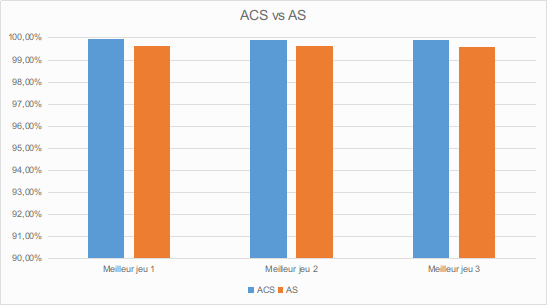
\includegraphics[width=\textwidth]{images/acsVSas.png}
\end{figure}

\paragraph{}
Comme le prévoyait l'aspect théorique, ACS est nettement supérieure en terme de taux de satisfiabilité à son homologue AS, cela est dû principalement au fait que ce dernier n'est pas une représentation fidèle  du comportement réel des fourmis, contrairement à ACS qui, par le bias de la marche aléatoire, se veut plus réaliste et représentatif de la vie réelle. bien que la différence est négligeable, cela reste une comparaison a petite échelle, dans les cas réels les instances sont beaucoup plus complexes et difficiles à résoudre.
%talk about how BSO is amazing

\part{Comparaisons et conclusions générale}
\chapter{Comparaisons des trois approches}
\chapter{Conclusion générale}
\paragraph{}
%Talk about the good sides of BSO and its bad sides, talk about the potential that resides in the metaheuristics and swarm intelligence.
\listoffigures
\listoftables
\bibliography{biblio.bib}
\appendix
\chapter{Code source}
\begin{figure}[H]
	\centering
	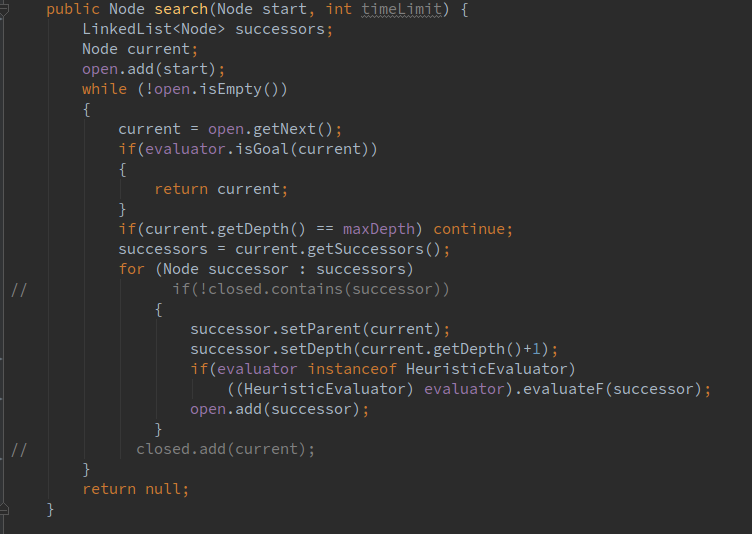
\includegraphics[width=\textwidth]{images/imgs/graphSearch.png}
	\caption{Algorithme de recherche principal}
\end{figure}

\begin{figure}[H]
	\centering
	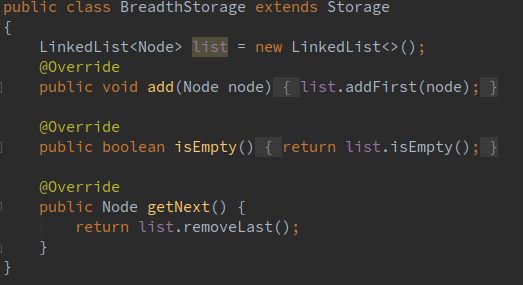
\includegraphics[width=\textwidth]{images/imgs/BFSstorage.png}
	\caption{Gestion de open en largeur d'abord}
\end{figure}

\begin{figure}[H]
	\centering
	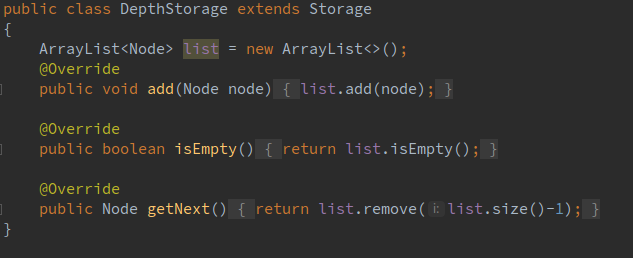
\includegraphics[width=\textwidth]{images/imgs/DFSStorage.png}
	\caption{Gestion de open par profondeur d'abord}
\end{figure}

\begin{figure}[H]
	\centering
	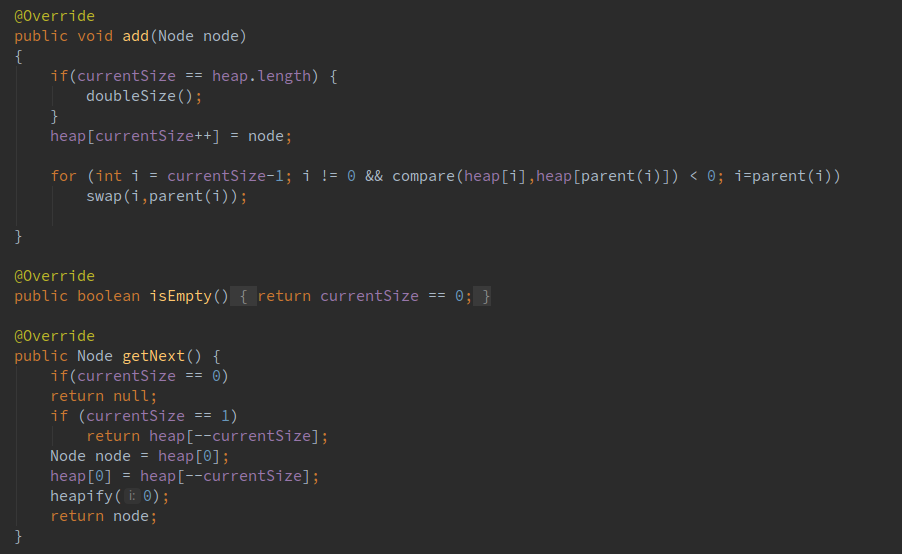
\includegraphics[width=\textwidth]{images/imgs/heapStorage.png}
	\caption{Gestion de open en tant que tas}
\end{figure}

\begin{figure}[H]
	\centering
	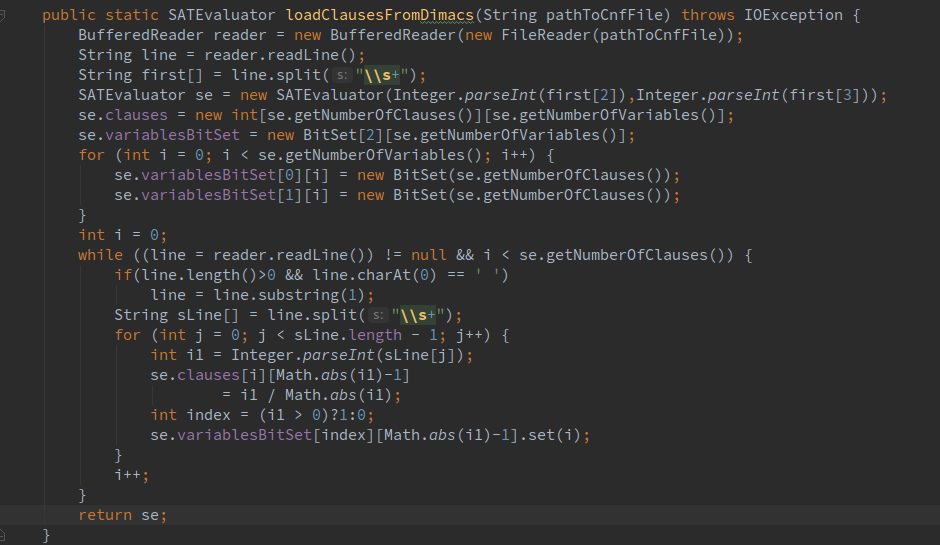
\includegraphics[width=\textwidth]{images/imgs/loadFromDimacs.png}
	\caption{Chargement de l'instance depuis le fichier benchmark}
\end{figure}

\begin{figure}[H]
	\centering
	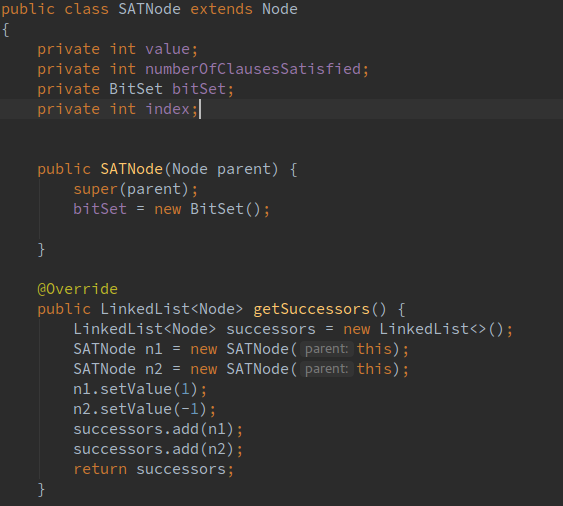
\includegraphics[width=\textwidth]{images/imgs/nodeStruct.png}
	\caption{Structure d'un noeud dans l'arborescence}
\end{figure}
\end{document}}\grid
